% siminos/spatiotemp/chapter/integLatt.tex
% $Author: predrag $ $Date: 2021-08-22 23:33:53 -0400 (Sun, 22 Aug 2021) $

\section{Lattice points enumeration}
\label{sect:integLatt}

\renewcommand\speriod[1]{{\ensuremath{L_{#1}}}}  %continuous spatial period
\renewcommand\period[1]{{\ensuremath{T_{#1}}}}  %continuous time period

% https://en.wikipedia.org/wiki/Leopold_Kronecker
\begin{bartlett}{
%Die ganzen Zahlen hat der liebe Gott gemacht, alles andere ist Menschenwerk"
God made the integers, all else is the work of man.
       }
\bauthor{
Leopold Kronecker}
\end{bartlett}


\subsection{Complex plane}

\HREF{https://en.wikipedia.org/wiki/Gaussian_integer} {wiki}:
{\em Gaussian integers} have many nice properties (factorization, primes, etc)
but I do not feel the complex plane relevant to our problem; for us
it is only the $d=2$ case of general lattice point counting of the next section..

\begin{description}

\item[2020-01-23 Predrag].

\HREF{https://en.wikipedia.org/wiki/Fundamental_pair_of_periods} {wiki}:
A {\em fundamental pair of periods} is a pair of complex numbers
\(\omega_1,\omega_2 \in \complex\) such that, considered as vectors in
\(\reals^2\), the two are not collinear. The lattice generated by
$\omega_1$ and $\omega_2$ is
\[
\lattice=\{m\omega_1+n\omega_2 \,\,|\,\, m,n\in\mathbb{Z} \}
\]
The two generators $\omega_1$ and $\omega_2$ are called the \emph{lattice
basis}. The parallelogram defined by the vertices 0, \(\omega_1\) and
\(\omega_2\) is called the \emph{fundamental parallelogram}, see
\reffig{fig:FundParall}.
The fundamental parallelogram contains no further lattice points in its
interior or boundary. Conversely, any pair of lattice points with this
property constitute a fundamental pair, and furthermore, they generate
the same lattice.

%By Alvaro Lozano Robledo - http://planetmath.org/?op=getobj&from=objects&id=4613, CC BY-SA 3.0,
%   https://commons.wikimedia.org/w/index.php?curid=5585978
\begin{figure}
  \centering
  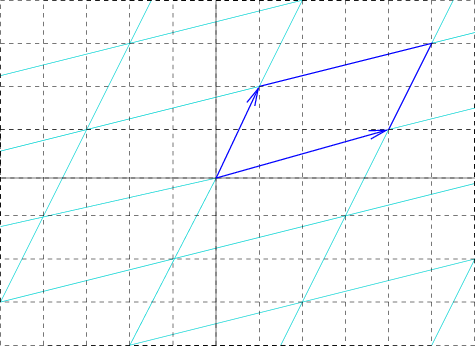
\includegraphics[width=0.40\textwidth]{Fundamental_parallelogram}
  \caption{\label{fig:FundParall}
A fundamental parallelogram spanned by (4,1) and (1,2) contains
${\Det \lattice = 7}$
points. Note that the far vertices (4,1), (1,2)  and (5,3) are not
counted, as they belong to other tiles.}
\end{figure}

A fundamental parallelogram spanned by (4,1) and (1,2) contains
\[
\Det\begin{pmatrix}
             4 & 1 \\
             1 & 2
      \end{pmatrix} = 7
\]
points, see \reffig{fig:FundParall}.

There is no unique fundamental pair; an infinite number of fundamental
pairs correspond to the same lattice. Any pair of fundamental
parallelograms is related by a modular group matrix
\(\in{SL}n{2}{\integers}\).  This equivalence of lattices underlies
many of the properties of elliptic functions (especially the Weierstrass
elliptic function - I think not relevant to us) and modular forms.

The abelian group \(\mathbb{Z}^2\) maps the complex plane
into the fundamental parallelogram. That is, every point \(z \in
\complex\) can be written as \(z=p+m\omega_1+n\omega_2\)
for integers $m$, $n$, with  a point $p$ in the fundamental
parallelogram.

If one identifies opposite sides of the parallelogram as
being the same, the fundamental parallelogram has the topology of a
torus; the quotient manifold
\(\complex/\lattice\) is a torus.
We are
possibly interested in functions on $\complex/$(lattice), functions on
$\complex$ with a certain periodicity condition. These doubly periodic,
meromorphic functions are called \emph{elliptic}.

\end{description}

\subsection{Integer lattice in $d$ dimensions}

Since we are interested in combinatorial rather than metric properties,
it suffices to consider the case of the standard integer lattice
$\integers^d\subset\reals^d$. The case of a general lattice \lattice\ in
$\reals^d$ reduces to that of $\integers^d$ by a change of the
coordinates.

\begin{description}

\item[2020-01-23 Predrag].

\HREF{https://en.wikipedia.org/wiki/Lattice_(group)} {wiki}:
{\em Lattice (group)}:
A lattice \lattice\ in \(\reals^d\)
has the form
\[
\lattice = \left\{\left. \sum_{i=1}^d a_i v_i \; \right\vert \; a_i \in\mathbb{Z} \right\}
\]
where
\beq
\{v_1,v_2,\cdots,v_d\}
\ee{integBas}
is a basis (or `integral basis') that defines the Bravais cell.
One convention is that an integral basis is ordered according to the
length of its elements; i.e. $|v_1|\leq|v_2|\leq\cdots\leq|v_d|$.

\HREF{https://en.wikipedia.org/wiki/Lattice_graph} {wiki}:
{\em A lattice graph},
mesh graph, or grid graph, is a graph whose drawing, embedded in
 $\reals^d$, forms a regular tiling.
In $d=2$ a lattice graph (or a square grid graph)
is the graph whose vertices correspond to the points in the plane with
integer coordinates.

The determinant (`discriminant' or `volume') of lattice $\lattice$ is
\beq
d(\lattice) = |\det(v_1|v_2|\cdots|v_d)|
\,.
\ee{lattVol}
The determinant is the reciprocal of the average density of points in the
lattice.
Different bases can generate the same lattice,
but the absolute value of the determinant
is uniquely determined by $\lattice$.
If one thinks of a lattice as dividing the whole of
\(\reals^d\) into equal polyhedra (copies of
an $d$-dimensional parallelepiped, the 'fundamental
region' of the lattice), then d($\lattice$) is equal to the $d$-dimensional
volume of this polyhedron.  This is why d($\lattice$) is sometimes called the
\emph{covolume} of the lattice.  If it equals 1, the lattice is called
unimodular.

The master of counting integer lattice points in various domains (and all
dimensions) is Alexander \HREF{http://www.math.lsa.umich.edu/~barvinok/}
{Barvinok}.
Barvinok \HREF{http://www.math.lsa.umich.edu/~barvinok/lectures.pdf}
{lectures} are very clear and simple. On p.~20 he defines the fundamental
parallelepiped, and then shows that

\textbf{Theorem 2}. The number of integer points in the fundamental
parallelepiped is equal to the volume of the parallelepiped.

Note that the fundamental parallelepiped is half-open, as indicated by
dashed lines in \reffig{Barvinok02fig81} so that the its translates form
a partition of the whole space.

Barvinok\rf{Barvinok02}
{\em A Course in Convexity}, \CBlibrary{Barvinok0}

Barvinok\rf{Barvinok08}
{\em Integer Points in Polyhedra}, \CBlibrary{Barvinok08} seems to
be a harder read, and not helpful for our integer lattice points counting.

1831 pages \HREF{http://www.csun.edu/~ctoth/Handbook/HDCG3.html}
{Handbook of Discrete and Computational Geometry} might be of some use.

\begin{figure}
  \centering
  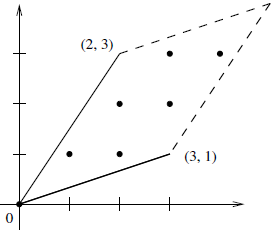
\includegraphics[width=0.35\textwidth]{Barvinok02fig81}
  \caption[]{\label{Barvinok02fig81}
A parallelepiped spanned by (3,1) and (2,3) contains
$\Det\begin{pmatrix}
             3 & 2 \\
             1 & 3
      \end{pmatrix} = 7$
points. Note that (3,1), (2,3) and the far vertex (5,4) are not counted.
Barvinok\rf{Barvinok02}~ Fig.~81.
  }
\end{figure}


Hademard's inequality.
Let $v_1,v_2,\cdots,v_d$ be any basis for $\lattice$. Then
\beq
d(\lattice)\leq |v_1| |v_2|\cdots|v_d|
\,,
\ee{reducedBas}
as the volume of a parallelepiped is
never greater than the product of the lengths of its sides. Hadamard's
inequality is an equality if and only if the basis vectors are orthogonal.
A theorem of Hermite says that every lattice has a basis that is
reasonably orthogonal (see \refeq{Holmin12-Hermite}), where the amount of
nonorthogonality is bounded solely in terms of the dimension. A
\emph{reduced basis} is an integral basis that minimizes the product of
lengths \refeq{reducedBas} over all bases of the lattice. Lattice
$\lattice$ is \emph{bounded} by T, if it has a reduced basis consisting of
vectors of length at most T.

\HREF{https://www.math.ucdavis.edu/~latte/software/packages/latte_current/manual_v1.7.2.pdf}
{LattE} is an ``Lattice point Enumeration'' program that  count  lattice
points  contained  in convex polyhedra defined by linear equations and
inequalities with integer coefficients\rf{DeLHTY04}. In 1994
Barvinok\rf{Barvinok94} gave an algorithm that counts lattice points in
convex rational polyhedra in polynomial time when the dimension of the
polytope is fixed. LattE counts the lattice points using multivariate
generating functions $P(a)$, $z^a=z^{a_1}z^{a_2}\cdots{z^{a_d}}$,
implementing Barvinok algorithm. At the end, $f(P)$ is written as a sum
of ``short'' rational functions.

Latte \HREF{https://www.math.ucdavis.edu/~latte/} {home page}.

\HREF{https://www.math.ucdavis.edu/~totalresidue/} {Maple} code.

Simplicial cone: Let \refeq{integBas} be a set of $k$ linearly
independent integral vectors in $\reals^d$, where $k\leq{d}$. Consider
simplicial cone $K$ and parallelepiped $S$ generated by \refeq{integBas},
\beq
K=\{\lambda_1 v_1+\lambda_2 v_2+\cdots+\lambda_k v_k\}
\,,\qquad 0\leq\lambda_i
\ee{coneK}
\beq
S=\{\lambda_1 v_1+\lambda_2 v_2+\cdots+\lambda_k v_k\}
\,,\qquad 0\leq\lambda_i<1
\ee{coneK1}
The generating function for the lattice points in $K$
equals\rf{Stanley09I}
    \PC{2020-01-25} {
I cannot find this formula in Stanley \rf{Stanley09I}, \CBlibrary{Stanley09I}.
    }
\beq
\sum_{\beta\in{K}\cap\integers^d}z^\beta=
\left(\sum_{\tau\in{S}\cap\integers^d}z^\tau\right)\prod_{i=1}^k \frac{1}{1-z^{v_i}}
\ee{coneKgenF}
A unimodular cone is a simplicial cone with all $\lambda=1$ which forms
an integral basis for the lattice
$\reals\{v_1,v_2,\cdots,v_k\}\cap\integers^d$. In this case the numerator
of the formula has a single monomial; in other words, the parallelepiped
has only one lattice point. The number of points in the parallelepiped
is obtained by
setting $z_i=1$ in the generating function
\beq
f(S;z)= \left(\sum_{\tau\in{S}\cap\integers^d}z^\tau\right)
\ee{noPinS}
However, the generating function is not constructed by enumerating all
the integer points in $S$, but rather as a signed sum of rational
functions that can be derived from the description of $S$. They all count
points in a general polyhedron; counting them in a parallelepiped should
be a simple special case, but I have not seen that discussed separately.

Note that this count does not identify opposing sides of the
parallelepiped.

If we need to enumerate periodic points one-by-one, John Voight
\HREF{https://mathoverflow.net/questions/57773/listing-lattice-points-in-a-simplex}
{mathoverflow} question might be a start.

\HREF{http://www.stumblingrobot.com/2015/07/15/prove-a-formula-for-the-area-of-a-polygon-whose-vertices-are-lattice-points/}
{Stumbling Robot} derives the area of a polygon whose vertices are
lattice points.

The study of integer points in convex polyhedra is motivated by questions
such as "how many nonnegative integer-valued solutions does a system of
linear equations with nonnegative coefficients have" or "how many
solutions does an integer linear program have".

\HREF{https://en.wikipedia.org/wiki/Minkowski\%27s_theorem} {wiki}:
{\em Minkowski's theorem} relates the number $d(\lattice)$ and the volume of
a symmetric convex set $S$ to the number of lattice points
contained in $S$. The number of lattice points contained in a
polytope all of whose vertices are elements of the lattice is
described by the polytope's Ehrhart polynomial. Formulas for some of
the coefficients of this polynomial involve $d(\lattice)$ as well.

\HREF{https://en.wikipedia.org/wiki/Ehrhart_polynomial} {wiki}:
An integral polytope has an associated {\em Ehrhart polynomial} that
encodes the relationship between the volume of a polytope and the number
of integer points the polytope contains. A generating function for the
Ehrhart polynomials, or the Ehrhart series is a rational function - this
suggest that we should able to convert this series into a zeta function.
This wiki has some intriguing explicit examples.

\item[2020-09-18 Predrag]
Subramaniam and Balani have an
\HREF{http://home.iitk.ac.in/~anandh/E-book/} {E-book}
with a cute chapter on
\HREF{http://home.iitk.ac.in/~anandh/E-book/lattice.ppt} {lattices},
but it standard Bravais lattice crystallography, of no use to us. Ignore

\item[2020-07-31 Predrag]
The \catlatt\ \jacobianOrb\ \refeq{catalattLxT}
in the {\HillDet} $\det{\jMorb}$ computation for a
$\BravCell{\speriod{}}{\period{}}{0}$ rectangular Bravais cell is
expressed naturally and spacetime symmetrically in terms of `horizontal',
`vertical' translation generators $\shift_{1}$, $\shift_{2}$.

I expect that for an arbitrary Bravais cell, such as
\reffig{Barvinok02fig81}, the corresponding translation generators should
act along the `integral basis' vectors \refeq{integBas} that define the
Bravais cell $\lattice$, \ie, the \catlatt\ {\HillDet} should be given by
\beq
\det{\mathbf{\jMorb}}=\det({\mathbf{\jMorb}\lattice)}/\det{\lattice}
\,,
\ee{HillDetAnyCell}
where \catlatt\ \jacobianOrb\ ${\mathbf{\jMorb}}$ should be expressed in
terms of translations along the Bravais cell basis vectors, and the
{\HillDet} should be expressed terms of invariant quantities that can be
constructed from them. The simplest is the volume \refeq{lattVol}, the
others are presumably related to traces $\tr\lattice^k$ and the
corresponding subvolumes. Not sure what they are, but someone has surely
thought about that. My understanding is summarized in
\HREF{http://birdtracks.eu/version9.0/GroupTheory.pdf\#section.6.4}
{birdtracks.eu}.

Han and I have an answer of asymmetric form for the \jacobianOrb\
\refeq{catalattLxT} for a tilted Bravais domain (\rpo)
\refeq{catalattLxTrop}, with the relative periodicity all in the
`comoving frame' translation generator
$\shift_{1}^{-\tilt{}/\period{}}\otimes\shift_2$.

This space-time asymmetry is a consequence of choosing the Hermite normal
form \refeq{Holmin12-Hermite} to define the Bravais cell. So - even
though we are computing the representation-independent determinants, we
do not have an invariant statement of cell's `tilt'. There must be a more
elegant answer to this.
Some of this discussion is in the {\bf 2020-07-11 Predrag} post,
around eq.~\refeq{DudMer84(2.106)}.

But that might lead us too deep into the role that prime numbers play in
characterizing equivalent Bravais cells $\lattice$ and their volumes.
Whenever you result depends on factorization in primes, it is time to
sound a potentially deep number theory {\color{red}red alert :)}

\item[2020-01-23 Predrag]
\HREF{https://cims.nyu.edu/~regev/} {Oded Regev} is good on this - will
post more links. He uses
Micciancio and Goldwasser\rf{MicG0l02}
{\em Complexity of Lattice Problems - A Cryptographic Perspective}
\CBlibrary{MicG0l02} as
his course textbook.

\HREF{https://cims.nyu.edu/~regev/teaching/lattices_fall_2004/ln/introduction.pdf}
{Oded Regev}: Definition~5 defines $d(\lattice)$, the determinant of a
lattice in terms of the Bravais basis that might be useful to us.

\HREF{https://cs.nyu.edu/courses/spring13/CSCI-GA.3033-013/}
{Lattices, Convexity and Algorithms} lecture notes from
\HREF{https://cs.nyu.edu/courses/spring13/CSCI-GA.3033-013/lectures/lecture-1.pdf}
{2013} might be better. Check out
``Gram Schmidt Orthogonalization,'' which I think is his construction
of the Hermite normal basis, and
``Equivalence of Lattice Definitions.''
Also check out his {\em Fundamental Parallelepiped and the Determinant}
\HREF{https://cs.nyu.edu/courses/spring13/CSCI-GA.3033-013/lectures/lecture-3.pdf}
{lecture}.

\item[2020-12-12 Predrag]                                          \toCB
Haviv and Regev \arXiv{1311.0366} address the Lattice Isomorphism
Problem (LIP). I like their definitions.

Two lattices $\lattice_1$ and $\lattice_2$ are
isomorphic if there exists an orthogonal linear transformation
mapping $\lattice_1$ to $\lattice_2$.

An {\em orthogonal} linear transformation (or {\em isometry}) $O : V_1
\rightarrow V_2$ is a linear transformation that preserves inner
products, that is, $\langle x, y\rangle = \langle O(x), O(y)\rangle$ for
every $x,y \in V_1$. For a set $A \subseteq V_1$ we use the notation
$O(A) = \{ O(x) \mid x \in A\}$.

For a matrix $B$ we denote its $i$th column by $b_i$, and $O(B)$ stands
for the matrix whose $i$th column is $O(b_i)$.
${\mathop{\mathrm{span}}}(B)$ stands for the subspace spanned
by the columns of $B$.

%\label{fact:Gram}
Let $B$ and $D$ be two matrices satisfying $B^T \cdot B = D^T \cdot D$.
Then there exists an orthogonal linear transformation
$O:{\mathop{\mathrm{span}}}(B) \rightarrow {\mathop{\mathrm{span}}}(D)$
for which $D = O(B)$.

An $m$-dimensional {\em lattice} $\lattice \subseteq \R^m$ is the set of
all integer combinations of a set of linearly independent vectors
$\{b_1,\ldots,b_n\} \subseteq \R^m $, i.e.,
$\lattice=\{\sum_{i=1}^{n}{a_i b_i}~|~\forall i.~a_i \in \integers\}$. The set
$\{b_1,\ldots,b_n\}$ is called a {\em basis} of $\lattice$ and $n$, the
number of vectors in it, is the {\em rank} of $\lattice$. Let $B$ be the
$m$ by $n$ matrix whose $i$th column is $b_i$. We identify the matrix and
the basis that it represents and denote by $\lattice(B)$ the lattice that
$B$ generates.
% The norm of a basis $B$ is defined by $\|B\| = \max_{i}{\|b_i\|}$.



A basis of a lattice is not unique: two bases $B_1$
and $B_2$ generate the same lattice of rank $n$ if and only if $B_1 = B_2
\cdot U$ for a {\em unimodular} matrix $U \in \integers^{n \times n}$,
i.e., an integer matrix satisfying $|\det(U)|=1$.

The determinant of a lattice $\lattice$ is defined by
\beq
\det(\lattice)=\sqrt{\det(B^T B)}
\,,
\ee{detLat}
where $B$ is a basis that generates $\lattice$.
$\det(\lattice)$ is independent of the choice of the basis. A
set of (not necessarily linearly independent) vectors that generate a
lattice is called a {\em generating set} of the lattice.

A lattice ${\cal M}$ is a {\em sublattice} of a lattice $\lattice$ if
${\cal M} \subseteq \lattice$, and it is a {\em strict sublattice} if
${\cal M} \subsetneq \lattice$. If a lattice $\lattice$ and its
sublattice ${\cal M}$ span the same subspace, then the {\em index} of
${\cal M}$ in $\lattice$ is defined by $|\lattice : {\cal M}| =
\det({\cal M})/\det(\lattice)$. If ${\cal M}$ is a sublattice of
$\lattice$ such that $|\lattice : {\cal M}|=1$ then ${\cal M}=\lattice$.

They define lattices by their \emph{Gram matrices}.
The {\em Gram matrix} of a matrix $B$ is defined to be the matrix
\beq
G = B^T \cdot B
\,,
\ee{Gram1}
or equivalently,
\beq
G_{ij} = \langle b_i , b_j \rangle
\,,\qquad \mbox{for every } i \mbox{ and } j
\,.
\ee{Gram2}
A Gram matrix specifies a basis only up to rotation.
\index{Gram matrix}

In the Lattice Isomorphism Problem the input consists of two Gram
matrices $G_1$ and $G_2$, and the goal is to decide if there exists a
unimodular matrix $U$ for which $G_1 = U^T \cdot G_2 \cdot U$.

The {\em dual lattice} of a lattice $\lattice$, denoted by $\lattice^*$,
is defined as the set of all vectors in
${\mathop{\mathrm{span}}}(\lattice)$ that have integer inner product with
all the lattice vectors of $\lattice$, that is,
\[
\lattice^* = \{u \in
{\mathop{\mathrm{span}}}(\lattice)~|~\forall v \in \lattice.~\langle u,v
\rangle \in \integers \}
\,.
\]
The {\em dual basis} of a lattice basis $B$ is
denoted by $B^*$ and is defined as the one which satisfies $B^T \cdot B^*
= I$ and ${\mathop{\mathrm{span}}}(B)={\mathop{\mathrm{span}}}(B^*)$,
that is, $B^* = B(B^T B)^{-1}$. It is well known that the dual basis
generates the dual lattice, i.e., $\lattice(B)^* = \lattice(B^*)$.

The relations between parameters of lattices and parameters of their dual
are known as {\em transference theorems}.

\item[2020-02-14 Predrag]
Given a nondegenerate lattice $\lattice$, we can construct an invariant by
choosing a basis, and taking the determinant of the matrix whose (i,j)
entry is the inner product of the i-th basis vector with the j-th basis
vector. The matrix is called the Gram matrix of the basis, and the
determinant is a rough measure of how loosely packed the lattice vectors
are in $\lattice\otimes\mathbb{R}$.

\item[2020-02-14 Predrag]
I have run (once) into `fundamental parallelepiped' being called
`fundamental parallelotope'.

\item[2020-12-12 Predrag]
For our choice of Hermite normal form \refeq{Holmin12-Hermite2d},
\refeq{HermiteBasis}, the {Gram matrix} \refeq{Gram1} is
\beq
G =
\left[\begin{array}{cc}
\speriod{}^2      & \speriod{}\tilt{} \\
\speriod{}\tilt{} & \speriod{}^2  + \period{}^2
\end{array}\right]
\,.
\ee{Gramin2d}

\item[2020-09-08 Predrag]
%\HREF{https://cseweb.ucsd.edu/classes/wi12/cse206A-a/lec1.pdf} 2012 course
\HREF{http://cseweb.ucsd.edu/classes/sp14/cse206A-a/lec1.pdf} % 2014 course
{Daniele Micciancio} is very economical. I propose we follow his exposition, and
use Micciancio and Goldwasser\rf{MicG0l02} {\em Complexity of Lattice
Problems - A Cryptographic Perspective} \CBlibrary{MicG0l02}. They
say (I have not looked at any of these, so they might be even better
than Micciancio and Goldwasser, for our purposes):

``Classical references about lattices are Cassels\rf{Cassels59} (or 1971)
\CBlibrary{Cassels59} and Gruber and Lekerkerker\rf{GruLek87}
\HREF{http://ChaosBook.org/library/GruLek871.djv} {(click here)}. Another
very good reference is Siegel\rf{Siegel89} \CBlibrary{Siegel89}. For a
brief introduction to the applications of lattices in various areas of
mathematics and science the reader is referred to (Lagarias 1995) and
(Gritzmann and Wills 1993), which also touch some complexity and
algorithmic issues. A very good survey of algorithmic application of
lattices is (Kannan 1987a).''

Lattices are regular arrangements of points in Euclidean space.  The
simplest example of lattice inn-dimensional space is $\integers^d$, the
set of all $d$\dmn\ vectors with integer entries. More generally, a
lattice is the result of applying a nonsingular linear transformation
$B\in{\reals^{m\times{d}}}$ to the integer lattice $\integers^d$, to
obtain the set
\(
B(\integers^m) =\{Bx:x\in \integers^d\}
\,.
\)
etc. - you fill it in.

To Han: can you replace our `Bravais' by Micciancio and
Goldwasser\rf{MicG0l02} lattice definitions?

Is the `Hermite
normal form'the same as the `Gram-Schmidt orthogonalization method'?

\item[2020-09-11 Han]
See \refsect{s:BravaisLatt}.
Gram Schmidt Orthogonalization constructs orthogonal with
basis vectors whose tips are not on $\integers^d$ lattice; not Hermite
normal form, forget it.


    	\HLpost{2018-01-31}{
The similarity transformation ${\bf S}$ that maps \refeq{ArnoldCat}
into \refeq{PerViv:2confRepMat},
\beq
{\bf A}
=\MatrixII{2}{1}
          {1}{1}
\,,\qquad
{\bf B}
=\MatrixII{0}{1}
          {-1}{3}
\,,
\ee{HLsimilarityB}
is
\beq
{\bf B} = {\bf S}^{-1}{\bf A}{\bf S}
\,,
\ee{HLsimilarityC}
where
\[
{\bf S} = {\bf S}^{-1}
        =\MatrixII{-1}{2}
				   {0}{1}
\,.
\]
}

\PCpost{2018-04-27}{
    % mathematica Matrix[{-1,2},{0,1}] Matrix[{1,1},{1,0}] Matrix[{-1,2},{0,1}]
Note that $\det {\bf S} = -1$. Why? That can be fixed by multiplying it
by $\ii$, but why? It is also not unique, one could,  for example, use
\[
{\bf S'} = {\bf S'}{}^{-1}
        =
\MatrixII{0}{-1}
		  {1}{0}
\MatrixII{-1}{2}
		  {0}{1}
\MatrixII{0}{1}
		{-1}{0}
        =
\MatrixII{1}{ 0}
		{-2}{-1}
\,.
\]
For a systematic discussion, see sect.~4. {\em Global versus local conjugacy
and orbit statistics} of Baake \etal\rf{BaRoWe08}, and sect.~2.5.  {\em
Results for d = 2} of Baake \etal\rf{BaNeRo13} {\em Orbit structure and
(reversing) symmetries of toral endomorphisms on rational lattices}. The main
point (for us) is that maps that are in the same conjugacy class need to have
3 invariants in common; the trace, the determinant, and the mgcd (the matrix
greatest common denominator). For the Thom-Arnol'd cat map \refeq{ArnoldCat},
$mgcd(A) = 1$

Baake \etal\rf{BaNeRo13} discus ``pretails''
to \po s at length.
}

\PCpost{2018-04-27}{
Next, one can transform Arnold cat map ``square root'' ${\bf C}$ (or,
according to Baake \etal\rf{BaRoWe08}, the `classic'' or golden orientation
reversing cat map, or the Fibonacci cat map\rf{BaNeRo13}, with $\det(\bf
C)=-1$)
\beq
{\bf A}={\bf C}^2\,,\qquad
{\bf C} = \MatrixII
 {1} {1}
 {1} {0}
\ee{AABHM99-44HL}
to the \PV\ version
\beq
{\bf B} = {\bf \tilde{C}}^2
\,,\quad
{\bf \tilde{C}} = {\bf S}^{-1}{\bf C}{\bf S}
 = \MatrixII
 {-2} {1}
 {-1} {1}
\,.
\ee{HLsimilarityS}
As noted in \refeq{AABHM99-46}, taking this ``square root'' expresses the
zeta function as a product of a time-reversal pair of zeta's. ${\bf B}$ and
${\bf\tilde{C}}$ have the same eigenvectors, but as $\det {\bf\tilde{C}}=-1$,
one of the stability multipliers is a negative square root of the ${\bf B}$
multipliers \refeq{catEigs},
\beq
\tilde{\ExpaEig} = \tilde{\ExpaEig}_1 = \frac{1 + \sqrt{5}}{2} % = 2.6180
\,,\qquad
\tilde{\ExpaEig}_2 = \frac{1 - \sqrt{5}}{2} % = 2.6180
\,.
\ee{goldenMltpl}
The issue of reversibility seems complicated\rf{BaNeRo13}.
When $M\in\mbox{SL}(2,\integers)$, also its inverse is in
$M^{-1}\in\mbox{SL}(2,\integers)$, and $M$ and $M^{-1}$ share the same determinant,
trace and mgcd:
\[
{\bf M} = \MatrixII
 {a} {b}
 {c} {d}
\,,\qquad
{\bf M}^{-1} = \MatrixII
 {~d} {-b}
 {-c} {~a}
\,.
\]
The the golden (Fibonacci\rf{BaNeRo13}) cat map \refeq{AABHM99-44HL} is not
reversible in $\mbox{GL}(2,\integers)$ (while its square $A$
is\rf{BaNeRo13}).
}



\PCpost{2020-02-19}{
\emph{Linear recurrences with constant coefficients: the multivariate case}
by
Mireille Bousquet-M{\'e}lou1a and Marko Petkov{\v{s}}ek,
\HREF{https://doi.org/10.1016/S0012-365X(00)00147-3} {(DOI)}
has the right feel and a few 2\dmn\ integer lattice recurrences and
the corresponding functional equations,
but I do not see how to apply it to the 2\dmn\ \catlatt.
    }

\item[2020-07-11 Predrag]
Woods\rf{Woods12} (2012) \CBlibrary{Woods12} is very clear, what follows
is excerpted from it. As Woods says, his starting chapters are taken
from Lim\rf{Lim90} {\em Two-dimensional Signal and Image Processing}
\CBlibrary{Lim90} \CBlibrary{BecRob07}, who copies from Dudgeon and
Mersereau\rf{DudMer84} (1984) {\em Multidimensional Digital Signal
Processing} \CBlibrary{DudMer84} which cover the same ground.
\\

A 2{\dmn} field $\field_{n \zeit}$ is periodic with period
$\BravCell{\speriod{}}{\period{}}{0}$, if the
following equalities hold for all integers $n$, $\zeit$:
\beq
\field_{n\zeit} = \field_{n + \speriod{}, \zeit}
                 = \field_{n, \zeit+ \period{}}
\,,
\ee{Woods12p6}
where \speriod{} and \period{} are positive integers.
This type of periodicity occurs often for 2{\dmn} signals and is referred to
as \emph{rectangular periodicity}. We call the resulting period the
\emph{rectangular period}.

Given a periodic function, the period effectively defines a basic cell in
the plane, which can be repeated to form the function over all integers
$n$, $\zeit$. As such, we often want the minimum size unit cell for
efficiency of both specification and storage. In the case of the
rectangular period, we seek the smallest nonzero integers that will
suffice for $\BravCell{\speriod{}}{\period{}}{0}$ to form this basic
cell.

\textbf{Horizontal Wave.}
Consider the sine wave
\(
\field_{n\zeit}  = \sin(2\pi n/4)
\,.
\)
The horizontal period is $\speriod{}=4$. In the vertical direction, the
signal is constant, so we can use any positive integer $\period{}$.
The smallest such value is $\period{}=1$. Thus the rectangular period is
$\BravCell{\speriod{}}{\period{}}{0}=\BravCell{4}{1}{0}$,
and the basic cell consists of the set of points
\(
\{({n\zeit}) = [(0,0),(1,0),(2,0),(3,0)]\}
\)
 or any translate of this set.

In general,  `periodicity' refers to a repetition of blocks, not
necessarily rectangular blocks or blocks occurring on a rectangular
repeat grid, with the periodicity represented with two integer vectors,
\[
v_1=\begin{pmatrix}
  \speriod{}\\
  c_{21}{}
  \end{pmatrix}
  \,,\qquad
v_2=\begin{pmatrix}
  \tilt{}\\
  \period{}
  \end{pmatrix}
  \,.
\]
While they note the nonuniqueness of Bravais cells with respect to
unimodular transformations, image processing textbooks seem not to use
the Hermite normal form \refeq{Holmin12-Hermite} to eliminate $c_{21}$.

The 2{\dmn} field $\field_{n \zeit}$ is periodic with period
\(
(v_1,v_2) = \Lambda
\)
if the following hold for all integers  $n$, $\zeit$:
\beq
\field_{n\zeit} = \field_{n + \speriod{}, \zeit+c_{21}}
                 = \field_{n + \tilt{}, \zeit+ \period{}}
\,,
\ee{Woods12p8}
To avoid degenerate cases, restrict the integers in $v_j$ with the
condition
\[
\det(v_1,v_2)\neq0
\,.
\]
``We leave it to the reader to show that'' the number of samples in this
region is $\det\Lambda$, \ie, the absolute value of the determinant of
the periodicity matrix gives the number of samples of $\field_{{\bf n}}$
contained in one period.

The matrix $\Lambda$ is called the \emph{periodicity matrix}. In matrix
notation, the periodic field satisfies
\[
\field_{{\bf n}} = \field_{{\bf n}+\Lambda{\bf r}}
\,,\qquad {\bf r}= \begin{pmatrix} r_{1}\\r_{2}\end{pmatrix}
\,.
\]
Two integer vectors ${\bf m}$ and ${\bf n}$ are \emph{congruent} with
respect to the matrix modulus $\Lambda$ if
\(
{\bf m}= {\bf n} + \Lambda{\bf r}
\)
for some integer vector ${\bf r}$.

In the case that $\Lambda$ is a diagonal
matrix, $\field_{{\bf n}}$ is \emph{rectangularly periodic}.

If $P$ is any integer matrix, then $P\Lambda$ is also be a periodicity
matrix for $\field_{{\bf n}}$. Thus the periodicity matrix is not unique
for any periodic sequence.

A matrix $E$ for which $\det E = 1$ is called a \emph{unimodular matrix}.
$E^{-1}$ is then also a unimodular matrix. Unimodular matrices are the
only integer matrices whose inverses are also integer matrices. If
$\det\Lambda$ is a prime number, we will say that $\Lambda$ is a
\emph{prime matrix}. If $\Lambda$ is neither prime nor unimodular, we say
that it is \emph{composite}, and can be decomposed, nonuniquely - up to
a unimodular transformation - into a
product of two non-unimodular matrices
    \index{unimodular matrix}
\beq
\Lambda=PQ
\,.
\ee{DudMer84(2.106)}
If either $P$ or $Q$ is composite, one continues the process, until
$\det\Lambda$ is the product of its prime factors.

Dudgeon and Mersereau\rf{DudMer84} then explain clearly how to get the
``quotient'' $Q$ when ``dividing'' by $P$. $|\det\Lambda|/|\det Q| =
|\det P|$ is then the number of cosets. In the image-processing, Fourier
transforms trade this non-prime factorization is known as
``decimation-in-time Cooley-Tukey FFT algorithm,'' ``twiddle factors,''
and ``butterflies.''
     \PC{2020-07-15} {
     Use this to define prime factorization in \refref{CL18}?
     }

{\bf Example} \Reqv\ field
\(
\sin [2\pi (n/8+\zeit/16)]
\)
is constant along the line
\(
2n+\zeit=16
\,.
\)
The basis vectors are
\[
v_1=\begin{pmatrix}
  4\\8
    \end{pmatrix}
  \,,\qquad
v_2=\begin{pmatrix}
  ~1\\-2
     \end{pmatrix}
  \,,\qquad
\mbox{with } \det\Lambda=16
  \,.
\]

\textbf{Definition 1.1-1: Linear System} $[\cdots]$ \\

\textbf{Definition 1.1-2: Shift Invariance} $[\cdots]$

``Linear shift-invariant discrete systems are generally implemented using
difference equations. Although multidimensional difference equations
represent a generalization of 1\dmn\ difference equations, they are
considerably more complex and are, in fact, quite different. A number of
important issues associated with multidimensional difference equations,
such as the direction of recursion and the ordering relation, are really
not issues in the 1\dmn\ case.

$[\cdots]$ they define multidimensional recursive systems and consider
the issues associated with multidimensional difference equations;
$[\cdots]$  define the multidimensional Z-transform.
''
\\

\textbf{2{\dmn} Convolution}
If a system is \emph{linear shift-invariant} (LSI), then  $[\cdots]$
%
the field $h$ is called the LSI system's \emph{impulse response}.
 $[\cdots]$
He defines the 2{\dmn} convolution operator  $[\cdots]$

\textbf{Properties of 2{\dmn} Convolution or Convolution Algebra}  $[\cdots]$
All 5 properties of convolution hold for any 2{\dmn} fields $x, y$, and $z$,
for which convolution is defined (i.e., for which the infinite sums
exist). His Figure 1.1-9 illustrates a convolution.
\\

\textbf{Stability in 2{\dmn} Systems}
    \PC{2020-07-11}{I do not understand BIBO, but maybe we should?}
Stable systems are those for which a small change in the input gives a
small change in the output. We define bounded-input bounded-output (BIBO)
stability for 2{\dmn} systems analogously to that in 1{\dmn} system
theory. A spatial or 2{\dmn} system will be stable if the response to
every uniformly bounded input is itself uniformly bounded. For an LSI
system the condition is equivalent to the impulse response being
absolutely summable,
\beq
\sum_{k1,k2} |h_{k1,k2}| <\infty
\,.
\ee{Woods12(1.1-3)}

Sect.~1.2 \textbf{2{\dmn} discrete-space Fourier transform} The Fourier
transform is important in 1{\dmn} signal processing because it
effectively explains the operation of linear time-invariant (LTI) systems
via the concept of frequency response, \ie, the Fourier transform of the
system impulse response. While convolution provides a complicated
description of the LTI system operation, with the input at all locations
$n$ affects the output at all locations, the frequency response provides
a simple interpretation as a scalar weighting in the Fourier domain,
where the output at each frequency $\omega$ depends only on the input at
that same frequency. A similar result holds for 2{\dmn} systems that are
LSI.

{\bf 2020-07-15 Predrag} Note that the discrete Fourier transform of a
Bravais lattice always carries the prefactor $1/\det\Lambda$. Going back
involves a volume $(2\pi)^d$.

\textbf{Definition 1.2-1: 2{\dmn} Fourier Transform} $[\cdots]$
In the 2{\dmn} Fourier transform the frequency variable $\omega_1$ is
called \emph{horizontal frequency}, and the variable $\omega_2$ is called
\emph{vertical frequency}.
 $[\cdots]$
As $n$, $\zeit$ are integers, the 2{\dmn} Fourier transform is periodic
with rectangular period $2\pi\times2\pi$, and only needs be calculated
for one period, usually taken to be $[-\pi,\pi]\times[-\pi,\pi]$.

$[\cdots]$
the 2{\dmn} Fourier transform is a \emph{separable operator}, because it
can be performed as the concatenation of 1{\dmn} operations on the rows
followed by 2{\dmn} operations on the columns.

\textbf{Inverse 2{\dmn} Fourier Transform} $[\cdots]$ \\

\textbf{Fourier Transform of 2{\dmn} or Spatial Convolution}\\
\textbf{Theorem 1.211: Fourier Convolution Theorem} $[\cdots]$ \\

$[\cdots]$
As a 2{\dmn} or spatial LSI system is characterized by its impulse
response $h_{n,\zeit}$, its frequency response $H_{\omega_1,\omega_2}$ suffices to
characterize such a system. And the Fourier transform Y of the output equals the product
of the frequency response H and the Fourier transform X of the input. When the
frequency response H takes on only values 1 and 0, the system is an \emph{ideal filter},
filtering out some frequencies and passing others unmodified.
More generally, the term filter include all such LSI systems, and
has been extended to shift-variant and even nonlinear systems through the concept of
the Voltera series of operators.
    \PC{2020-07-11}{
`Voltera series of operators'? Defined in
S. Thurnhofer and S. K. Mitra, {\em A General Framework for Quadratic
Volterra Filters for Edge Enhancement}, IEEE Trans. Image Process., vol.
5, June, pp. 950-963, 1996.
    }

\textbf{Some Important Properties of the FT Operator} $[\cdots]$ \\

\textbf{Some Useful Fourier Transform Pairs} $[\cdots]$ \\

\textbf{Example 1.2-4: Fourier Transform of Separable Signal} $[\cdots]$ \\

\textbf{Symmetry Properties of the Fourier Transform} $[\cdots]$ \\

Generally, we think of the Fourier transform as the evaluation of the
Z-transform on the unit polycircle $\{|z_1| = |z_2| = 1\}$; however, this
assumes the polycircle is in the region of convergence of $X(z_1,z_2)$,
which is not always true.

  $[\cdots]$
linear shift-invariant systems with sinusoidal excitations are naturally
described by the Fourier transform. The Z-transform is a generalization
of the Fourier transform which allows us to treat exponential inputs.

  $[\cdots]$
Exponentials of the form $\ssp_{n_1 n_2} = z^{n_1}z^{n_2}$ are
eigenfuctions of 2\dmn\ linear shift invariant systems.

 The 2\dmn\ Z-transform of a discrete field \Xx\ is defined as
\beq
\Xx_{z_1z_2}^Z =
\sum_{n_1=-\infty}^{\infty}\sum_{n_2=-\infty}^{\infty}
 \ssp_{n_1 n_2} z_1^{-n_1}z_2^{-n_2}
%    \continue
%    \ceq
\,.
\label{DudMer84(4.18)}
\eeq

\textbf{Example 3.4-5: Comparison of Fourier Transform and Z-Transform}
$[\cdots]$ \\

The Fourier transform is not strictly a subset of the Z-transform,
because it can use impulses and other singularity functions, which are
not permitted to Z-transforms.

  $[\cdots]$
The Fourier transform is used primarily to describe signals and to
describe the actions that systems will have on them. The Z-transform is
used to describe systems and to provide an additional tool for
manipulating difference equations. While the 2\dmn\ Z-transform is related
to its l\dmn\ counterpart, the two transforms are actually quite
different.

For $z_1 = e^{i\omega_1}$, $z_2 = e^{i\omega_2}$ the Z-transform reduces
to the Fourier transform. The corresponding surface in the Z-domain is
the called 2\dmn\ unit \emph{bicircle}. 2\dmn\ Z-transform
converges on the \emph{Reinhardt domain}, the 2\dmn\  analog of the annulus
for 1\dmn\ case.
\\



\renewcommand\speriod[1]{{\ensuremath{\ell_{#1}}}}  %continuous spatial period
\renewcommand\period[1]{{\ensuremath{\ell_{#1}}}}  %continuous time period

\item[2020-02-23 Predrag]
Continuing on the multivariate generating functions,
the {\em integer-point transform} introduced in this
 textbook in integer lattices counting:
Beck and Robins\rf{BecRob07}
{\em Computing the Continuous Discretely},
\CBlibrary{BecRob07}, might be helpful:

% clip & paste from \arxiv{1509.03121}
Let ${\bf a} =(a_1,\dots ,a_d)$ $\in\integers^d$ be an integer point. The
Laurent monomial ${\bf z}^{\bf a}$  is defined as
\beq
{\bf z}^{\bf a}
:=z_1^{a_1}z_2^{a_2}\cdots z_d^{a_d}, \quad {\bf z}^{\bf{0}}:=1
\ee{BecRob07:LaurMon}
 where
${\bf{0}}:=(0,0,\dots ,0)$. For a given rational cone or rational
polytope $S\subset \reals^d$,
\beq
\sigma_S({\bf z})
    =\sigma_S(z_1,z_2,\dots ,z_d)
   :=\sum_{{\bf a}\in S\cap \integers^d}{\bf z}^{\bf a}
\ee{BecRob07:IntPoTrnsf}
is called the {\em integer-point transform} of $S$.
The function $\sigma_S$ lists all integer points in $S$ not as a
list of vectors, but as a sum of monomials. This
$\sigma_S$ also goes by the name \emph{moment generating function} or
simply \emph{generating function} of $S$.
    \index{integer-point transform}
    \index{moment generating function}\index{generating function}

%%%%%%%%%%%%%%%%%%%%%%%%%%%%%%%%%%%
\begin{figure}
  \centering
  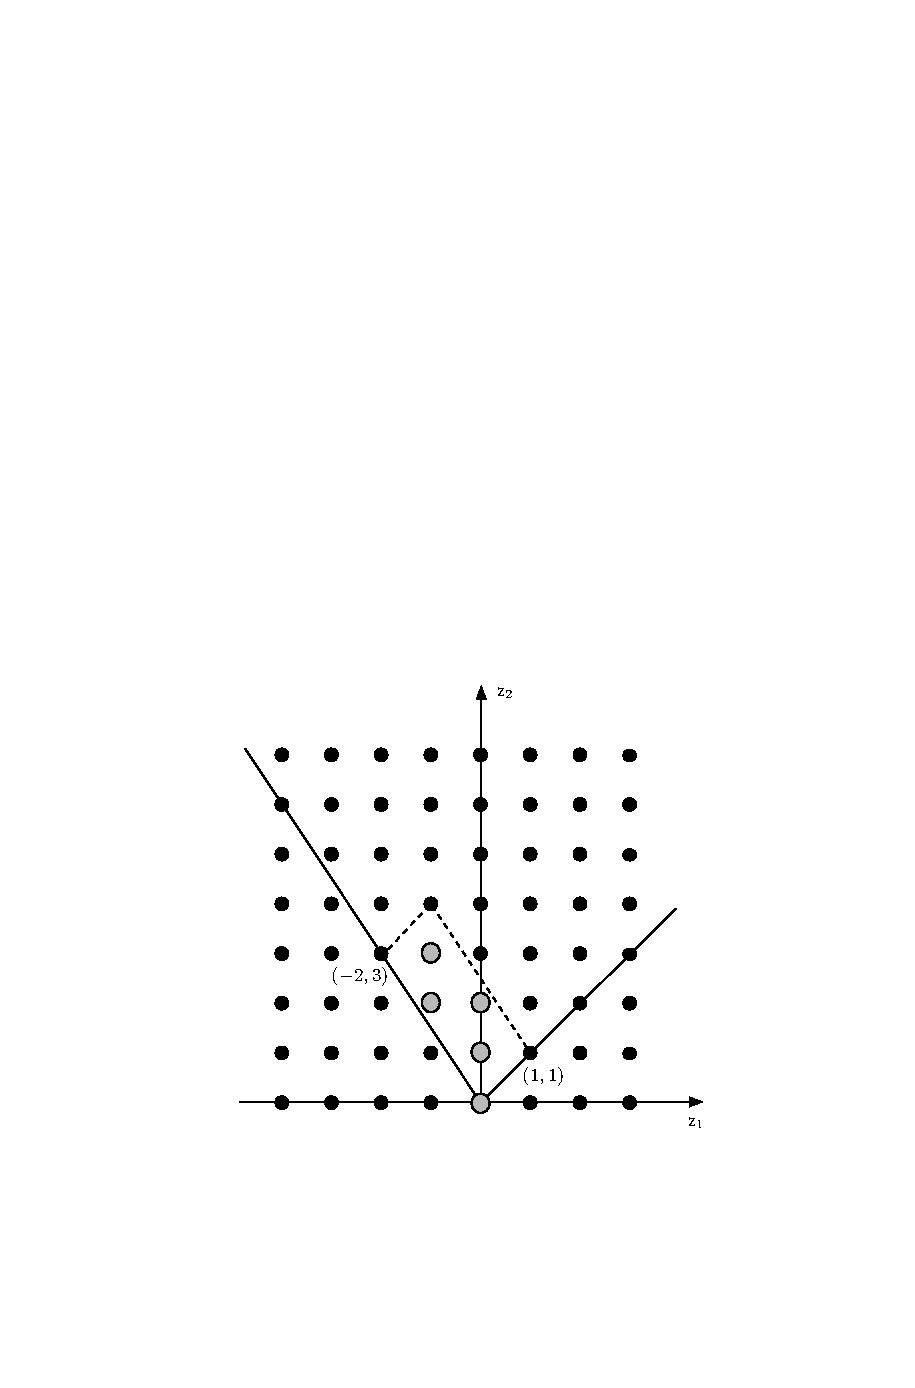
\includegraphics[width=0.40\textwidth]{BecRob07fig3-3}
  \caption{\label{BecRob07:fig3-3}
The cone ${\cal K}$ and its fundamental parallelogram,
fig~3.3 from \refref{BecRob07}.
    }
\end{figure}
%%%%%%%%%%%%%%%%%%%%%%%%%%%%%%%%%%%%

They start with the usual trivial example of a geometric series in
Example 3.3, and work out a 2\dmn\ $\{(1, 1),(-2, 3)\}$ Bravais lattice
in example Example 3.4, see \reffig{BecRob07:fig3-3}. They call the
$\reals^2$ interior of the half-open Bravais cell `fundamental
parallelogram $\Pi$', and tile the two-dimensional cone ${\cal K}$ with
its non-negative translations. That results in the rational polynomial
formula for the integer-point transform of the cone ${\cal K}$
\beq
\sigma_{\cal K}({\bf z}) =
\frac{1 + z_2 + z_2^2 + z_1^{-1}z_2^2 + z_1^{-1} z_2^3}
     {(1 - z_1z_2)(1 - z_1^{-2} z_2^3)}
\ee{BecRob07:examp3-4}
of the form that I had suggested to Han for
the \catlatt.
\medskip

Check also:
\begin{itemize}
  \item
{\bf 2020-03-02 Predrag} notes below, on Wilf\rf{Wilf94}
sect.~1.5 {\em Two independent variables}.
  \item
\emph{Characteristic function} or ``five-point stencil''
\refeq{FGHLW74:charFunct2d}
\end{itemize}


\item[2020-03-03 Predrag]
OK,
the {\fundPip} determinant \refeq{lattVol} counts integer points
\beq
N_\cl{} = |\Det\jMorb| = |\Det(v_1|v_2|\cdots|v_\cl{})|
\,.
\ee{eq:fundFact}
What does
\(
\Tr\jMorb
\)
do? That is also an invariant under $SLG(\cl{})$ lattice transformations.


\end{description}


\subsection{Primitive parallelogram}

\begin{description}

\item[2020-01-25 Predrag]

A lattice vector is called \emph{primitive},  if there is no other
lattice points on the segment between  0  and the tip.

or:

% from Holmin  	10.1007/s00605-013-0518-x,  	\arXiv{1211.2716}
An integer vector $v\in\integers^d$ is {\em primitive}
if it cannot be written as an integer multiple $m\neq 1$ of some other
integer vector $w\in\integers^d$.
\index{primitive vector}

or:

A lattice point is a primitive lattice point if it is not a multiple of any
other lattice point, that is, the greatest common divisor of its
coordinates is one.

or:

A primitive lattice point is a
lattice point visible from the origin.

Let $A$ be an integer $[d\times d]$-matrix with
nonzero determinant $k$ and primitive row vectors.
The common divisors of the entries of each row
of $A$ are preserved under multiplication on
the right by any matrix $X\in{SL}n{d}{\integers}$.

A lower triangular integer matrix
\beq
  C\defeq \begin{pmatrix}
  c_{11}&0&\cdots&0\\
  c_{21}&c_{22}&\ddots&0 \\
  \vdots&&\ddots&0\\
  c_{d1}&\cdots&c_{d(d-1)}&c_{dd}
  \end{pmatrix}
\ee{Holmin12-Hermite}
is said to be in (lower) {\em Hermite normal form} if $0<c_{11}$ and
$0\leq c_{ij}<c_{ii}$ for all $j<i$.

 I would prefer the vectors to
be column vectors, as in Lind \refeq{HLreciprocal7}.
In particular, in the case of 2\dmn\ square lattice,
\renewcommand\speriod[1]{{\ensuremath{L_{#1}}}}  %continuous spatial period
\renewcommand\period[1]{{\ensuremath{T_{#1}}}}  %continuous time period
\beq
  C\defeq \begin{pmatrix}
  \speriod{}&\tilt{}\\
  0&\period{}
  \end{pmatrix}
\ee{Holmin12-Hermite2d}
The Bravais cell basis column vectors are
\[
v_1=\begin{pmatrix}
  \speriod{}\\
  0{}
  \end{pmatrix}
  \,,\qquad
v_2=\begin{pmatrix}
  \tilt{}\\
  \period{}
  \end{pmatrix}
  \,,
\]
where $0\leq S<\speriod{}$ is the relative-periodic `shift,' or `screw'
for a screw-boundary condition, and our convention is $\speriod{}\geq\period{}$,
the rest obtained by discrete symmetries.

\renewcommand\speriod[1]{{\ensuremath{\ell_{#1}}}}  %continuous spatial period
\renewcommand\period[1]{{\ensuremath{\ell_{#1}}}}  %continuous time period

Orbit of $\Lambda$, a matrix in
Hermite normal form with primitive row vectors,
is denoted $\{A\Lambda|A\in{SL}n{2}{\integers}\}$.

\noindent{\bf Lemma}[Cohen\rf{Cohen93}, Theorem 2.4.3]
%\label{lemma_hnf}
Assume $k>0$. Given an arbitrary matrix $A\in M_{n,k}$, the orbit
$A{SL}n{d}{\integers}$ contains a unique matrix  $\Lambda$ in Hermite normal form.


\HREF{https://www.diva-portal.org/smash/get/diva2:874875/FULLTEXT01.pdf}
{Samuel Holmin} PhD thesis\rf{Holmin15} is a user-friendly overview of
his papers, such as {\em Counting nonsingular matrices with primitive row
vectors}\rf{Holmin13} \arXiv{1211.2716}.
Holmin defines a \emph{primitive} parallelogram: ``Consider a
parallelogram with integer coordinates which cannot be decom\-posed into
smaller parallelograms with integer coordinates. We will call such an
object a primitive parallelogram; see \reffig{Holmin15-Fig1} for an
illustration. How many primitive parallelograms are there with an area of
10? There are infinitely many such primitive parallelograms: in fact,
starting with a single primitive parallelogram, we can produce another
one with the same area by for example shifting it an integer distance up
or to the right, or by shearing it, % (see Figure 1.2),
and by repeating
either of these operations we can produce arbitrarily many different
parallelograms, all of which are primitive and have the same area.''

Curiously, even though in his 2nd papers he mentions that different
Bravais cells correspond to the same {\em lattice}, his
claim of \reffig{Holmin15-Fig1} is wrong.

%Figure 1.1 -
\begin{figure}
  \centering
  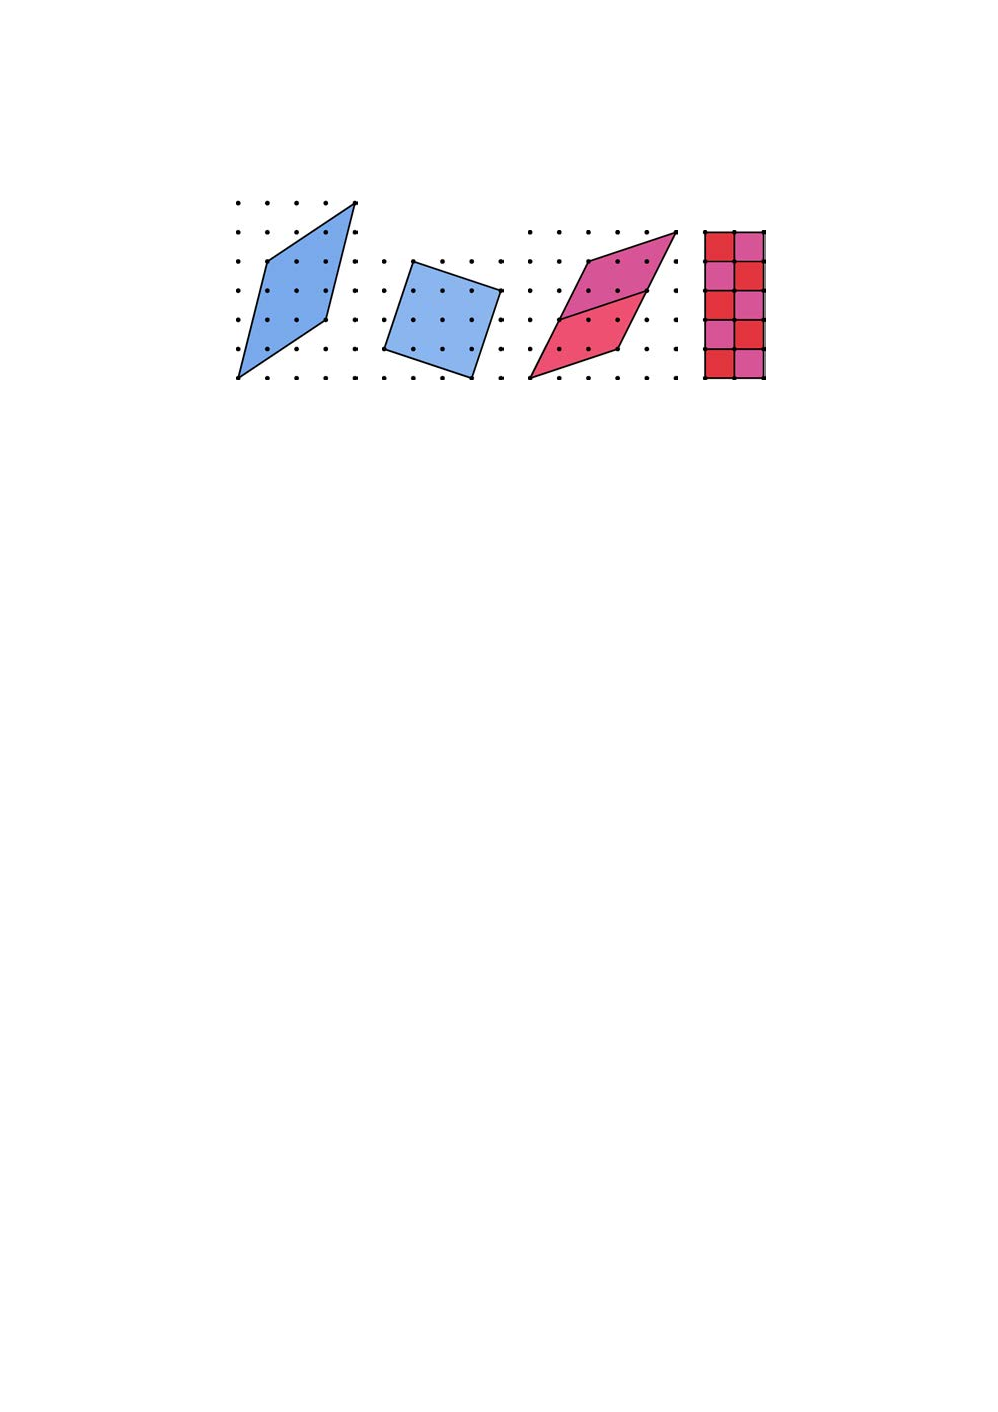
\includegraphics[width=0.60\textwidth]{Holmin15-Fig1}
  \caption{
Four Bravais cells of area 10, a figure from Holmin's PhD thesis\rf{Holmin15}.
The two blue Bravais cells are not
`primitive' (\ie, prime), as they are clearly
tiled by smaller prime Bravais cells.
Homlin claims that the two blue Bravais cells are
primitive, but that is wrong, see \refeq{Holmin15-Fig1HL}.
          }\label{Holmin15-Fig1}
\end{figure}

Wigman\rf{Wigman05}
{\em Counting singular matrices with primitive row vectors}: ``
Let us consider the set of singular $[n\times{n}]$ matrices with integer
entries. We are interested in the question how many among these matrices
have primitive row vectors, that is each row is not a nontrivial multiple
of an integer vector. We count the matrices according to the maximal
allowed Euclidean length of  the  rows.  Without  the  constraint  of
primitivity  the  problem  of  counting  such matrices  was  solved  by
Katznelson~[??].''

Wigman\rf{Wigman05} and Katznelson focus on asymptotic counting, which
we probably do not need.

\item[2020-02-19 Predrag]
Alexander Gorodnik
\HREF{https://www.math.uzh.ch/gorodnik/ds17/DynSysErgThPartI_17-18.pdf}
{lecture notes} discuss cat map $(A^n-\unit)$ and says
``The number of such solutions is exactly the area $\det(A^n-\unit)$ of
{\fundPip} in virtue of the

\textbf{Pick's theorem} (Gorodnik's Theorem 1.5.3, and A.4.1).
Let $i$ be the number of points with integer coordinates in the interior
of parallelogram $P$ and $b$ be the number of points with integer
coordinates on the perimeter of $P$. Then, Area$(P) =i+(b/2)+1$, with
points on the edges are counted as half and all vertices count as a
single point.

He proves the theorem. As usual, Pick's theorem is for $\reals^2$, not
general enough for us.

\item[2020-02-19 Predrag]
Baake, Hermisson and Pleasants\rf{BaHePl97}
{\em The torus parametrization of quasiperiodic {LI}-classes}
call this theorem a ``Fundamental  fact'' (their eq.~(10)), and
prove it, in Appendix for $d$\dmn\ tori maps, \ie,
in the case that we need. They use it to count all manner of tilings.
What they emphasize, and what we might have to
pay attention to, is the structure of the symmetry solutions on
$\mathbb{T}^d$.

\item[2020-02-21 Predrag]
Jezierski and Marzantowicz\rf{JezMar06}
\CBlibrary{JezMar06} write:

let $f:X \to X$ be a self-map of a set X.\\
(1.0.4) Definition. If $x \in X$ is a periodic point of f then any $m \in
N$ such that fm(x) = x is called a period of x. The smallest period of x
is called the minimal period of x with respect to f. The set of all
minimal periods of $x \in X$ is called the set of minimal periods of f
and denoted by Per(f).

We will define the fundamental algebraic invariants of a map f which
allow us to study the following notions:

\begin{itemize}
  \item Lefschetz number L(f) (cf. (2.3.12)), correspondingly Lefschetz numbers
{L(fm)} of all iterations and their algebraic combinations, informing about
the existence of fixed, respectively periodic points.
  \item Nielsen number N(f) (cf. (4.1.2)), correspondingly Nielsen periodic numbers
NFm(f) (cf. (5.1.16)), NPm(f) (cf. (5.1.14)) estimating from below
the number of fixed, respectively points of period m and m-periodic points.
\end{itemize}

[...]
This theory was initiated by Jakob Nielsen\rf{Nielsen1920} in 1920
% https://link.springer.com/content/pdf/10.1007/BF01457977.pdf
by the
observation that every self-map of the two-dimensional torus
$f:\mathbb{T}^2\to \mathbb{T}^2$  has at least |det(I-A)| fixed points
(here $I, A\in  M_{2{\times}2}(\integers)$ are respectively the identity
matrix and the matrix representing the induced homotopy homomorphism
$f_\#$ of $\pi_1(\mathbb{T}^2) = \integers^2$).

In 1975 R. Brooks, B. Brown J. Pak, and D. Taylor\rf{BBPT75}
derived a
nice formula for the Nielsen number $N(f)$ for the torus map: the Nielsen
number equals the absolute value of the Lefschetz number.
[...] The following theorem has been proved in \refref{BBPT75}.

(4.3.14) Theorem. For every self-map of the torus $f: \mathbb{T}^d \to
\mathbb{T}^d$, L(f) = det(I-A) and N(f) = |L(f)|.

Proof. Since the Lefschetz and Nielsen numbers are homotopy invariants we
may assume that $f = f_A$, i.e. f is induced by the linear map A.

\begin{enumerate}
  \item $f_A$ has exactly |det(I-A)| fixed points,
  \item no two fixed points of $f_A$ are Nielsen related,
  \item the index of each fixed point equals sgn(det(I-A)).
\end{enumerate}


[...] the fundamental theorem which allows us to extend the Nielsen fixed
point theory from tori into nilmanifolds. This theorem was proved
simultaneously by Anosov [An], and also Fadell and Husseini [FaHu2].

(6.3.13) Theorem. Let $f:X \to X$ be a self-map of a compact nilmanifold.
Then N(f) = |L(f)| and L(f) = det(I-A), where A denotes the
linearization matrix of f (cf. Definition (6.3.4), Proposition (6.3.6)).

\item[2020-02-22 Predrag]
Brooks \etal\rf{BBPT75}
{\em Nielsen numbers of maps of tori}:

If  $f:  X  \to X$  is  any  map on a $k$\dmn\ torus  X,  then the
Nielsen number and Lefschetz number of $f$  are  related by  the  formula
$N(f)=|L(f)|$.   Thus, on  the torus, the  Lefschetz number gives
information, not  just on  the existence of fixed points, but  on  the
number of  fixed points as  well. No  other compact Lie group has this
property.

\item[1995-09-08, 2020-12-08 Predrag]
Fel{'s}htyn and Hill\rf{FelHil95} {\em Trace formulae, {Zeta} functions,
congruences and {Reidemeister} torsion in {Nielsen} theory}
\arXiv{chao-dyn/9509009} paper is rich in examples of trace formulas and
zeta functions, but it's probably safe to ignore all this...

``
The Artin-Mazur zeta function and its modification count periodic points
of a map geometrically, the Lefschetz's type zeta functions do this
algebraically (with weight given by index theory). Another way to count the
periodic points is given by Nielsen theory.

The Lefschetz zeta function is always rational function of $z$ and is given by
a determinant formula. Manning\rf{manning} proved the rationality of the
Artin-Mazur zeta function for diffeomorphisms of a compact smooth manifold
satisfying Smale's Axiom A.

In Nielsen theory the `fixed point class' is determined by the `lifting
class'. A fixed point class is called \emph{essential} if its index is
nonzero. The number of lifting classes (and hence the number of fixed
point classes, empty or not) is called the \emph{Reidemeister Number}.
Generating functions for these numbers are called the Reidemeister zeta
and Nielsen zeta functions. They are homotopy invariants.
''

\end{description}


\subsection{Tensor eigenvalues}

In principle Han has solved the periodic states counting problem for
$d$\dmn\ hypercubic lattices by the discrete Fourier transform
diagonalization formula \refeq{HLreciprocal20}. A conceptual problem is
that the answer is stated in terms of $\cos$'s of rational angles, and it
is not obvious how those combine to yield an integer as the final result,
the number of periodic states.

For that reason it might be nice to perform the inverse Fourier transform
to the configuration space, to see what the basis vectors and the
fundamental parallelogram of the 2\dmn\ integer lattice look like, and
unify the treatment of the 1\dmn\ and higher\dmn\ lattice points
counting. We have looked at the relationship between the {\lattstate}s
and their Fourier representation in \refeq{FourierSpacePoints},
\reffig{fig:HLmtildeAndxtildeOf124Cycles},
\refeq{FourierCycPermT=4}, \etc.

Also we have some suggestive lattice solutions, such as
\refeq{HL2DimensionOrbit2}, \reffig{fig:HLAllPointsOf2By2Blocks}
(unit cube have been preferable - this is in the cube center coordiantes).

There is much literature on eigenvectors of tensors - probably we can
figure it out on our own, but I'm recording possible references just for
record here:

\begin{description}
\PCpost{2018-02-06}{
A job candidate Glen Evenbly talked about ``Tensor Networks'', (also
known as ``birdtracks'', but getting a citation out of computer nerds who
do it is harder than pulling teeth - at best I can pass under ``Penrose
diagrams''). If you want to see a lot of non-birdtracky pictures,
Rom{\'a}n Or{\'u}s \HREF{http://www.romanorus.com/DPGTutorial2014.pdf}
{has them}. Basically, if you are solving a 1D lattice problem, the
transfer operator is a matrix. However, if you are acting on a 2{\dmn} or
higher lattice, the transfer operator has pairs of more indices replacing
each index ow the 1D matrix, hence ``tensor.'' We need to understand that
as we go from cat map Toeplitz matrices to their $d$\dmn\
generalizations.
    }


\item[2020-02-14 Predrag]
Mateusz Micha{\l}ek and Bernd Sturmfels\rf{MicStu20}
{\em Invitation to Nonlinear Algebra},  \CBlibrary{MicStu20}
discuss symmetric $[n\!\times\!n]$ matrices tensor eigenvectors in Sect.~9.1.

The main monograph in this subject is
Qi, Chen and Chen\rf{QiChCh18}
{\em Tensor Eigenvalues and Their Applications},  \CBlibrary{QiChCh18}.

They find convenient to replace the n\dmn\ affine space  with the
(n-1)\dmn\ projective space, where two nonzero vectors are identified if
they are parallel.

Papers not looked at yet:

{\em All Real Eigenvalues of Symmetric Tensors}
\HREF{https://doi.org/10.1137/140962292} {DOI}:

{\em Generalized Tensor Eigenvalue Problems}
\HREF{https://doi.org/10.1137/140975656} {DOI}:

 {\em On determinants and eigenvalue theory of tensors}
\HREF{https://doi.org/10.1016/j.jsc.2012.10.001} {DOI}:

%{\em ##}
%\HREF{##} {DOI}:

%{\em ##}
%\HREF{##} {DOI}:

%\HREF{} {wiki}:

%\HREF{} {wiki}:


\end{description}


\section{Difference equations}
\label{sect:diffEqs}

\subsubsection*{sect.~2.3
                Linear homogenous equations with constant coefficients,
                Elaydi\rf{Elaydi05}}
% 2020-03-28 Predrag

Consider \emph{$k$th-order difference equation}
\beq
\field_{n+k} + p_1\,\field_{n+k-1} + p_2\,\field_{n+k-2}
             + \cdots + p_k\,\field_{n} = 0
\,,
\ee{Elaydi05(2.3.1)}
where $p_i$ are constants and $p_k\neq0$.
A $k$th-order difference equation with constant coefficients is often
referred to as $(k+1)$-term recurrence relation, see
\refsect{sect:genFuncts}.
Assuming a solution of form
$\field_{n}=\ExpaEig^n$ leads to the \emph{characteristic equation}
(see also `characteristic function' \refeq{FGHLW74:charFunct1d})
\beq
\ExpaEig^{k} + p_1\ExpaEig^{k-1} + p_2\ExpaEig^{k-2}
             + \cdots + p_k = 0
\,,
\ee{Elaydi05(2.3.2)}
with characteristic roots
\(
\{\ExpaEig_{1},\ExpaEig_{2},\cdots,\ExpaEig_{k}\}
\,.
\)
If the roots are distinct,
\[
\{\ExpaEig_{1}^\cl{},\ExpaEig_{2}^\cl{},\cdots,\ExpaEig_{k}^\cl{}\}
\]
is a set of fundamental solutions, and the general solution is of form
\beq
\field_{\cl{}}  = \sum_{i=1}^{k} a_i\ExpaEig_{i}^\cl{}
\,,
\label{Elaydi05(2.3.4)}
\eeq
where constants $a_i$ are determined by the initial conditions
$\{\field_{0},\field_{1},\cdots,\field_{k-1}\}$.


If the roots are not distinct, one also has fundamental solutions
of form $\cl{}^m\ExpaEig_{i}^\cl{}$.

\subsubsection*{sect.~2.4
                Linear inhomogenous equations,
                Elaydi\rf{Elaydi05}}
% 2020-03-28 Predrag

\beq
\field_{n+k} + p_1\,\field_{n+k-1} + p_2\,\field_{n+k-2}
             + \cdots + p_k\,\field_{n} = g_{n}
%\,,
\ee{Elaydi05(2.4.4)}
represents a physical system in which the \emph{forcing term}
(or \emph{external force}, or \emph{control}, or \emph{input}) $g_{n}$
is the input, and $\field_{n}$ the output,
\[
g_{n} \to \mbox{ system } \to \field_{n}
\,.
\]
The solutions of \refeq{Elaydi05(2.4.4)} do not form a vector space, \ie,
their linear combinations are not also solutions. However, a difference
of any pair of solutions is a solution of the homogenous difference
equation \refeq{Elaydi05(2.3.1)}, and a general solution of the linear
inhomogenous system \refeq{Elaydi05(2.4.4)} is a sum of the
\emph{complementary} solution (a homogenous solution $\field_{c}$ of
\refeq{Elaydi05(2.3.1)}, and a \emph{particular} solution $\field_{p}$
\beq
\field_{n} = \field_{c,n} + \field_{p,n}
%\,,
\ee{Elaydi05(2.4.3)}
A simple example of a particular solution: if $g_{n}=a^n$, then
$\field_{p,n}=c_1a^n$.

\bigskip

\begin{description}
\item[2020-03-28 Predrag]
There are many books on difference equations. \\
I like
Elaydi\rf{Elaydi05} \CBlibrary{Elaydi05}, but I have also downloaded\\
% Woods\rf{Woods12}
% {\em Multidimensional signal, image, and video processing and coding}
% \HREF{http://ChaosBook.org/library/Woods12} { (click here)}\\
Kelley and Peterson\rf{KelPet01} \CBlibrary{KelPet01}\\
Agarwal\rf{Agarwal00} \CBlibrary{Agarwal00}\\
Agarwal\rf{Agarwal06} \CBlibrary{Agarwal06}\\
Allen, Aulbach, Elaydi and Sacker\rf{AAES05} \CBlibrary{AAES05}\\
Galor\rf{Galor07} \CBlibrary{Galor07}\\
Ozisik, Orlande, Colaco and Cotta\rf{OOCC17} \CBlibrary{OOCC17}\\
Micciancio and Goldwasser\rf{MicG0l02}\\
% {\em Complexity of Lattice Problems - A Cryptographic Perspective}

\item[2020-04-13 Predrag]
Dannan, Elaydi and Liu\rf{DaElLi00}
{\em Periodic solutions of difference equations}
is a treasure trove of results on periodic solutions of difference equations:
marginal eigenvalues, Floquet exponents and multipliers,
Fredholm alternative.

    \item[2020-08-10 Predrag]
Lick\rf{Lick89} {\em Difference Equations from Differential Equations}
\CBlibrary{Lick89} we probably do not need.

The most general, quasi-linear, second-order PDE in two independent
variables is his eq.~(2.0.2). Depending on coefficients, the equation can
be \emph{hyperbolic}, such as the $d=2$ spacetime wave equation (2.0.3).
He focuses on \emph{parabolic} (${s}=2$ for us), such as the time
dependent diffusion equation given by (2.0.4).

Elliptic equations usually describe the steady-state limit of problems
where the time-dependent problem is described by parabolic or hyperbolic
partial differential equations. The most common elliptic equation is
$d=2$ space`time' symmetric Laplace's equation (2.0.5).

He defines Helmholtz equation (4.0.5),
 Laplace's equation (4.0.6), and Poisson's equation (4.0.7).
 His emphasis is on the discretized Helmholtz equation (4.1.3).

Sect.~2.4 {\em Algorithms for Two-Dimensional Problems}
has the 5-term recurrence, his eq.~(2.4.3) and (4.1.3).

Difference equations arising from elliptic equations generally
necessitate the solution of a large set of linear algebraic equations.
The matrix corresponding to this set of equations is generally sparse and
good solution methods take advantage of this fact.
[...]
the direct solution of these difference equations is quite time
consuming. When the number of equations is large, iterative methods of
solution are usually more efficient.

(4.2.8) defines \emph{Jacobi iteration}, a method of improving initial
guess solution.
(4.2.9) method is known as Gauss-Seidel iteration or the method of
successive relaxation.



\item[2016-07-11 Predrag]
%\subsection{Martin / Martin06}\label{sect:Martin06}
Boris cites P. A. Martin\rf{Martin06} {\em Discrete scattering theory: {Green}'s
function for a square lattice}

The \emph{lattice Green's function} is the main subject of the paper.

We consider the simplest problem, with a two-dimensional, square lattice.
Each lattice point can move out of the plane of the lattice, and that each
point is connected to its neighbours by springs; only nearest-neighbour
interactions are included. This leads to a system of partial difference
equations. The same equations are obtained if the two-dimensional Helmholtz
equation is discretized using the central-difference approximation (lattice
d'Alembert operator) for the Laplacian.

\item[2017-09-11 Predrag]
Morita\rf{Morita71} {\em Useful procedure for computing the lattice
{Green's} function - square, tetragonal, and bcc lattices}: `` A
recurrence relation, which gives the values of the lattice Green's
function along the diagonal direction from a couple of the elliptic
integrals of the first \refeq{Cserti00(38)} and second kind, is derived
for the square lattice by an elementary partial integration. The values
of the square lattice Green's function at an arbitrary site are then
calculated in a successive way with the aid of the difference equation
defining the function.
''
The method yields a recursion formula for a peculiar lattice Green's function
on a 2d lattice, but not the LGF itself.


\item[2017-09-09 Predrag]
Simons\rf{Simons97}
uses \refeq{Elaydi05(2.3.4)} in his \refeq{YamAbd97fundSol} to
invert a particular banded matrix.

See also \refexam{exam:TentLCod}~{\em Tent map linear code.}

Compare {characteristic equation} \refeq{Elaydi05(2.3.2)} to the
characteristic function $a(z)$ \refeq{FGHLW74:charFunct1d}.

\end{description}

\subsection{Time quasilattices}
\label{sect:timeQuasiLatt}

{\bf 2018-10-10, 2020-03-12 Predrag} Felix Flicker writes:
``My student Leon Zaporski and I have been investigating the
topological entropy of substitution sequences in the symbolic dynamics of
periodic orbits in discrete-time dynamical systems. We were hoping you
might be willing to take a look at our draft,
Zaporski and Flicker\rf{ZapFli19} {\em Superconvergence of topological
entropy in the symbolic dynamics of substitution sequences},
\arXiv{1811.00331},
and to send any
thoughts you might have, both in terms of whether you think the results
would be of interest to the community, and if there is a journal you
might recommend for us to submit to.''
\begin{quote}
                                        \toCB
I failed to read it. But it needs to be included in ChaosBook, as well
as many of the references.
\end{quote}
Their Fig.~1 is the topological entropy as a function of a control
parameter of the logistic map\rf{PeCaCe94}.
[...]
In the cases that accumulation points correspond to generalised time
quasilattices, the Boyle-Steinhardt class\rf{BoySte16} is indicated above
the curve.
\begin{quote}
Predrag:
I made several attempts to get some kind
of renormalization theory for the Sharkovsky sequence, with no
interesting results to report. Dahlquist wrote up his attempt
\toChaosBook{section.R.1} {(click here)}.
\end{quote}
[...]
Period doubling continues to be of importance to cutting edge research:
recent experiments established the existence of (discrete) time crystals,
which spontaneously break the symmetry of a periodic driving by returning
a robust period-doubled response, made rigid to perturbations and finite
temperature by the local interactions of many degrees of freedom.
[...]
periodically-driven nonlinear systems can feature not just period-doubled
responses, but robust responses with the symmetries of one-dimensional
(generalised) \emph{time quasilattices}\rf{Flicker18}.
[...]
Quasilattice substitution rules fall within the set we consider, and, by
considering a simple generalisation of the basic quasilattice concept, we
find that we are able to identify aperiodic orbits corresponding to all
physically relevant quasilattices, extending previous results identifying
two cases. Generalizing further we consider a set of substitutions
additionally covering, for example, the period-doubling cascade.
[...]
Whereas the topological entropy is zero for all sequences in the
period-doubling cascade, for other substitution sequences it increases
monotonically.
[...]
We find that the topological entropy of the wide class of substitution
sequences we consider converges as a double exponential onto its
accumulation point.
[...]
We demonstrate that all one-dimensional quasilattices can appear as
stable orbits in nonlinear dynamical systems.

Here is something we might find useful for \catlatt:

[...]
we focus on the \emph{generalised composition rules}, which systematically
generate admissible words by a substitution process\rf{Bruijn81}.

[...]
The universal order of periodic windows coincides with the
\emph{parity-lexicographic order} of words, defined through the relation
`$\prec$' in the following way:
\[
L \prec C \prec R
\]
and for two admissible words they state it in a way that is perhaps
superior to                                         \toCB
\toChaosBook{section.14.5}{ChaosBook}. Cite it there.
\medskip

[...]
{\bf Word operations}
\begin{itemize}
\item $\bar{\mathbf{A}} \bar{\mathbf{B}}$ indicates the concatenation of words $\bar{\mathbf{A}}$ and $\bar{\mathbf{B}}$
\item $\lvert\bar{\mathbf{A}}\rvert$ returns the number of letters in $\bar{\mathbf{A}}$
\item $\lvert\bar{\mathbf{A}}\rvert_{R,L}$ returns the number of letters $R,L$ in $\bar{\mathbf{A}}$
\item $\bar{\mathbf{A}}\rvert_C$ substitutes the final letter of $\bar{\mathbf{A}}$ with the letter $C$.
\end{itemize}
%
Inverse words are defined as follows (Predrag - I do not understand this):
%
\begin{align}
\bar{\mathbf{A}}^{-1}\left(\bar{\mathbf{A}}\bar{\mathbf{B}}\right)=\bar{\mathbf{B}}\nonumber\\
\left(\bar{\mathbf{A}}\bar{\mathbf{B}}\right)\bar{\mathbf{B}}^{-1}=\bar{\mathbf{A}}.
\end{align}

\begin{theorem}\label{secorder} %
Substitution rules generating a cascade
with initial word $\bar{\mathbf{W}}_{1}=R$ and
$\bar{\mathbf{W}}_{2}=\bar{\mathbf{R}}$ can be restated as a second order
linear recursive relation
$\bar{\mathbf{W}}_{n+2}=g(\bar{\mathbf{W}}_{n},\bar{\mathbf{W}}_{n+1})$
under concatenation if
$\bar{\mathbf{W}}_{3}=g(\bar{\mathbf{W}}_{1},\bar{\mathbf{W}}_{2})$. %
\end{theorem}
[...]
Consider a $[2\times2]$ \emph{growth matrix}
\begin{align}
A=\left(\begin{array}{cc}
a & b\\
c & d
\end{array}\right)
\end{align}
which quantifies the growth in the numbers of each letter type:
\begin{align}
\left(\begin{array}{c}
\left|\bar{\mathbf{W}}_{n}\right|_R\\
\left|\bar{\mathbf{W}}_{n}\right|_L
\end{array}\right)\rightarrow\left(\begin{array}{cc}
a & b\\
c & d
\end{array}\right)\left(\begin{array}{c}
\left|\bar{\mathbf{W}}_n\right|_R\\
\left|\bar{\mathbf{W}}_n\right|_L
\end{array}\right)=\left(\begin{array}{c}
\left|\bar{\mathbf{W}}_{n+1}\right|_R\\
\left|\bar{\mathbf{W}}_{n+1}\right|_L
\end{array}\right)
\end{align}
The class of substitutions we consider
can then be written as
%
\begin{align}
\bar{\mathbf{W}}_{n}&=\bar{\mathbf{W}}_{n-1}\mathcal{P}\left(\bar{\mathbf{W}}_{n-1}^{\text{tr}\left(A\right)-1}\bar{\mathbf{W}}_{n-2}^{-\det\left(A\right)}\right)
\end{align}
%
for $n>2$, with $\bar{\mathbf{W}}_{1}=R$, and $\bar{\mathbf{W}}_{2}$
a specified word. The symbol $\mathcal{P}$ indicates an unspecified
permutation. The characteristic equation of the growth matrix $A$ is
%
\begin{align}
\lambda^{2}-\text{tr}\left(A\right)\lambda+\det\left(A\right)&=0
\,.
\label{eq:W_characteristic}
\end{align}
%
The eigenvalues of $A$  must be real, either integer or quadratic irrational
(when we consider quasilattices).
The ratio of the components of the eigenvector associated to the largest
eigenvalue gives the relative frequencies of the two cell
types\rf{BoySte16}.
Eq.~\eqref{eq:W_characteristic} can be seen as the $n\rightarrow\infty$
limit of the defining equation of some integer sequence $W_n$ given by
%
\begin{align}
W_{n}&=\text{tr}\left(A\right)W_{n-1}-\det\left(A\right)W_{n-2}
\end{align}
for $n>2$, $W_1=\left|\bar{\mathbf{W}}_1\right|=1$, and
$W_2=\left|\bar{\mathbf{W}}_2\right|$. The ratio $W_n/W_{n-1}$ gives the
best possible rational approximation, for denominators not larger than
$W_{n-1}$, to the largest eigenvalue of the growth matrix, \emph{i.e.}
the larger of the solutions to Eq.~\eqref{eq:W_characteristic}.

[...]
As an example, the period-doubling substitutions lead to
the integer sequence
%
\begin{align}
W_n=W_{n-1}+2W_{n-2}
\end{align}
%
for $n>2$, with $W_1=\left|\bar{\mathbf{W}}_1\right|=\left|R\right|=1$ and $W_2=\left|\bar{\mathbf{W}}_2\right|=\left|RL\right|=2$. Explicitly, the first few terms are
%
\begin{align}
1,\,2,\,4,\,8,\,16,\,32,\,64,\ldots
\end{align}
%
\emph{i.e.} $W_n=2^{n-1}$.
\begin{quote}
Predrag: This is perhaps related to $s=2$ version of
\refeq{Chen11:1stepDiffSolu}.
\end{quote}
Then they do Fibonacci.
[...]
The eigenvalues of a $[2\times2]$ growth matrix $A$ are real and given by
%
\begin{align}
\lambda_\pm=
\frac{1}{2}\left({s}\pm\sqrt{{s}^2-4\det{A}}\right)
\,,\quad
{s}=\tr{A}
\,.
\label{eq:characteristic}
\end{align}
%
If ${s}^2=4\det{A}$ they are integers. Otherwise,
the larger eigenvalue is a quadratic irrational `Pisot-Vijayaraghavan'
(PV) number: the largest root of an irreducible monic polynomial, all of
whose Galois conjugates have modulus strictly less than
one.
[...]
The three conditions are necessary and sufficient for the
substitutions to correspond to quasilattice inflation
rules\rf{BoySte16}:
\begin{enumerate}
\item the growth matrix must be unimodular, $\left|\det{A}\right|=1$
\item there must be two spacings between each symbol
\item the largest eigenvalue of the growth matrix must be a PV number.
\end{enumerate}
The condition $\left|\det{A}\right|=1$, implies the inverse of the growth
matrix is also an integer matrix. The
inflation (substitution) of any quasilattice sequence can therefore be
undone with a well-defined deflation. This endows quasilattices with a
discrete scale invariance\rf{BoDiFl20}.
The third, PV numbers condition is necessary for the
interpretation of the quasilattice sequence in terms of a cut through a
higher-dimensional regular lattice.

The concept of quasilattices
relating to higher-dimensional lattices is discussed at length in
\refrefs{BoySte16,Flicker18}. % ,FlickervanWezel15}.

\begin{quote}
Predrag: So our ${s}=3$ \templatt\ $\lambda^{2}-3\lambda+1=0$ eigenvalue
$\frac{3+\sqrt{5}}{2}$ turns out to be a PV number. So is
${s}=4$ \templatt\ $\lambda^{2}-4\lambda+1=0$ eigenvalue
$2+\sqrt{3}$.
Both are the Boyle-Steinhardt\rf{BoySte16} quasilattices, of class 1,
respectively 3.
\end{quote}
[...]
Starting from an orbit described by the word $R$, repeated application of
the inflation rules will lead to a cascade of stable periodic orbits of
increasing length. After an infinite number of substitutions, \emph{i.e.}
at the accumulation point of the sequence, lies a stable orbit described
by an aperiodic word: a \emph{time quasilattice}.
[...]
Characteristic equation
%
\begin{align}
\lambda^2=4\lambda-1.
\end{align}
leads to the (modulus of the)
Clapeyron numbers $C_n$ ($A125905$ in the
\HREF{https://oeis.org/} {On-Line Encyclopedia} of
Integer Sequences)
\begin{align}
C_n=4C_{n-1}-C_{n-2}
\end{align}
for $n>2$ with $C_1=1$, $C_2=4$.
\begin{quote}
Predrag: In conclusion, \templatt\ is related to counting
of quasilattice words. Not sure it is of any use to us.
\end{quote}


\begin{description}

\item[2020-04-12 Predrag] Have a look at
Flicker, Simon and Parameswaran\rf{FlSiPa20}
{\em Classical dimers on {Penrose} tilings}.
[...]
[...]
[...]
[...]
[...]
[...]
[...]
[...]
[...]

\end{description}



\section{Generating functions}
\label{sect:genFuncts}

(Note, there is also a totally unrelated Lagrangian `generating function',
\refsect{sect:GenFuncLit}, nothing to do with this section of the blog.)
\bigskip

{\bf Definition}\rf{BecRob07}.
Let $f(x)$ be a series in powers of $x$. Then by the
symbol $[x^n]f(x)$ we will mean the coefficient of $x^n$ in the series
$f(x)$.



\begin{description}

\item[2020-03-20 Predrag]                               \toCB
The theory generating function (AKA Z-transforms) is pedagogically
explained by Elaydi\rf{Elaydi05}, including a table of common
Z-transform pairs, in analogy with the familiar Laplace transform tables.

\item[2020-09-30 Predrag]                               \toCB
Online
\HREF{http://pilot.cnxproject.org/content/collection/col10064/latest/}
{Signals and Systems} has pedagogical chapters on Z-transforms.

\item[2020-07-11 Predrag]
Woods\rf{Woods12}
{\em Multidimensional signal, image, and video processing and coding},
Chap.~3 {\em Two-Dimensional Systems and Z-Transforms}
 (2012) \CBlibrary{Woods12}.

\item[2020-01-23 Predrag]
For multivariate
generating functions
\beq
N(z)\,,\qquad
z^n=z^{n_1}z^{n_2}\cdots{z^{n_d}}
\,,
\ee{genFuncts:multiVar}
see
\refeq{coneKgenF},
\refeq{BecRob07:LaurMon},
\refeq{BecRob07:IntPoTrnsf},
\refeq{BecRob07:examp3-4}
.

Other examples of generating functions:
\refeq{2ndChebGenF},
\refeq{Wu04:gen},
\refeq{eq:DetPfaffianRel}
.

\item[2020-04-07 Han]
\renewcommand\speriod[1]{{\ensuremath{L_{#1}}}}  %continuous spatial period
\renewcommand\period[1]{{\ensuremath{T_{#1}}}}  %continuous time period
Perhaps we need three generating function variables
\bea
N(z_1,z_2,z_3)
    & = &
\sum_{\speriod{}=1} N_{\BravCell{\speriod{}}{\period{}}{\tilt{}}}
   z_1^{\speriod{}}z_2^{\period{}} z_3^{\tilt{}}
%    \continue
%    \ceq
\,.,
\label{3varPerOrCount}
\eea
Here $z_3^{\tilt{}}$ sum is finite, $-\speriod{}<{\tilt{}}<\speriod{}$,
and that feels not sufficiently invariant, as it depends on Hermite normal form
convention. Need something invariant...
\renewcommand\speriod[1]{{\ensuremath{\ell_{#1}}}}  %continuous spatial period
\renewcommand\period[1]{{\ensuremath{\ell_{#1}}}}  %continuous time period

\item[2020-03-01 Predrag]
Cute but true; Wilf\rf{Wilf94} {\em Generatingfunctionology} defines
the periodic points counting generating function as
\beq
N(z) = \sum_{\cl{}\geq0} N_n z^n
\,,
\ee{Wilf94:genFunct}
and starts out in his sect. 1.1~{\em An easy 2-term recurrence}, with
our Bernoulli periodic points count (for the ${s}=2$ case only)
\beq
N_{\cl{}} = s^{\cl{}} - 1
\,,
\ee{genFuncts:noPerPtsBm}
as a trivial example of a two-term recurrence (first-order difference
equation\rf{Elaydi05})
\beq
N_{\cl{}+1} = 2\,N_{\cl{}} + 1 \,,\qquad (s=2;\cl{}\geq0, N_0=0)
\,,
\ee{Wilf94:noPerPtsBm}
and (Predrag's insert) for  ${s}\neq2$,
\beq
N_{\cl{}+1} - s\,N_{\cl{}} = (s-1) \,,\qquad (\cl{}\geq0, N_0=0)
\,,
\ee{genFuncts:noPerPtsBms}
and its conversion to the periodic points count generating function
\refeq{Wilf94:genFunct}.
For \refeq{Wilf94:noPerPtsBm} he derives and expands in partial fractions
\beq
N(z;2) = \frac{z}{(1-z)(1-2z)} =  \frac{2z}{1-2z} -  \frac{z}{1-z}
\,,
\ee{Wilf94:noPerPtsGF}
and (Predrag's addition) for ${s}\neq1$,
\beq
N(z;s) = ({s}-1)z + ({s}-1)({s}+1)z^2 + ({s}-1)({s}^2+{s}+1)z^3 + \cdots
\,,
\ee{Wilf94:noPerPtsGFs}
verifying the Bernoulli periodic points count
\refeq{genFuncts:noPerPtsBm}.
Take
\(
N_{\cl{}} = ({s}-1)\hat{N}_{\cl{}}
\,,
\)
then \refeq{genFuncts:noPerPtsBms} leads to
\beq
\hat{N}_{\cl{}+1}  -{s}\,\hat{N}_{\cl{}} = 1
 \,,\qquad
(\cl{}\geq0, \hat{N}_0=0, \hat{N}_1 = 1)
\,.
\ee{genFuncts:BernRec-s1}
\beq
\hat{N}(z;s) = z + ({s}+1)z^2 + ({s}^2+{s}+1)z^3 + \cdots
\,,
\ee{Wilf94:noPerPtsGFs1}
For $s=1$ this is a complicated way to generate integers.


Then he does, as an example of a 3-term recurrence
(second-order difference equation\rf{Elaydi05}),
the Fibonacci recurrence
\beq
F_{n+1} = F_{n}+F_{n-1}:  \,,\qquad (\cl{}\geq1, F_0=0, F_1 = 1)
\,,
\ee{Wilf94:FibRec}
and derives
\beq
N(z) = \frac{z}{1-z-z^2}
     =
\frac{1}{z^{-1}-1-z}
\,.
\ee{Wilf94:FibRecGF}
Here the expansion in partial fractions is
in terms of roots of the (`golden mean') polynomial
\(
1-z-z^2
\)
.

He notes that the Stirling numbers of the first kind satisfy a 3-term
recurrence relation.


\item[2020-06-20 Predrag]
Oscar Levin %\rf{Levin19}
{\em Discrete Mathematics: An Open Introduction}
\HREF{http://discrete.openmathbooks.org/dmoi3/sec_addtops-genfun.html}
{Sect.~5.1 Generating Functions} works out a 3-term recurrence
$a_n = 3a_{n-1} - 2a_{n-2}$, with $a_0=1,a_1=3$ in
Example 5.1.6.  Surprisingly, one gets again (!)
\[
a_n = 2^{n+1} - 1
\,.
\]

\item[2020-06-20 Predrag]
Check out also Al Doerr and Ken Levasseur
\HREF{http://faculty.uml.edu/klevasseur/ads/index-ads.html}
{{\em Applied Discrete Structures}}:

\HREF{http://faculty.uml.edu/klevasseur/ads/s-recurrence-relations.html}
{{\em Sect.~8.3 Recurrence relations}}.

\HREF{http://faculty.uml.edu/klevasseur/ads/s-generating-functions.html}
{{\em Sect.~8.5.2 Solution of a Recurrence Relation Using Generating Functions}}.

\item[2020-03-04 Predrag]
\HREF{http://www.maths.surrey.ac.uk/hosted-sites/R.Knott/Fibonacci/LRGF.html\#section2.1}
{Ron Knott} writes:

The series of natural numbers
$1, 2, 3, 4, \cdots$
has the generating function
\beq
\frac{1}{(1-z)^2}=\frac{1}{1-2z+z^2}
\ee{genFuncts:n}
and the 3-term  recurrence (second-order difference equation\rf{Elaydi05})
%\[
%\field_{n}=2\field_{n-1}-\field_{n-2}
%\]
%We can see the relationship more clearly if we rewrite the recurrence in this form:
\[
\field_{n}-2\field_{n-1}+\field_{n-2}=0
\]
and compare that with the denominator of the generating function, namely:
\[
1-2z+z^2
\]
which might be a way to understand why $s=2$ is special.

A variant of Fibonnaci:
0,1,3,8,21,...is generated by
\[
\frac{z}{z^2-3z+1}
=
\frac{1}{z-3+z^{-1}}
\]
which looks \templatt-like.

\item[2020-03-02 Predrag]
In sect.~1.4 {\em A three term boundary value problem} Wilf\rf{Wilf94}
considers a 3-term recurrence with Dirichlet \bcs
\beq
au_{n+1} + bu_{n} + cu_{n-1} = d_{n} \,,\qquad
(n = 1,2,...,N-1;u_0 = u_N = 0)
\ee{Wilf94(1.4.1)}
where the positive integer N, the constants a, b, c and the sequence
$\{d_n\}^{N-1}_{n=1}$ are given in advance. The eqs \refeq{Wilf94(1.4.1)}
determine the sequence $\{u_i\}^N_0$ uniquely. Such boundary value
problems arise in applications such as the interpolation by spline
functions.

\bigskip

\item[2020-03-01 Predrag]
Compare \refeq{genFuncts:noPerPtsBms} to our\rf{CL18} Bernoulli 1-step difference
condition
\beq
\field_{\zeit} - {s}\field_{\zeit-1} = - \Ssym{\zeit}
\,,\qquad  \field_{\zeit} \in [0,1)
\,.
\ee{genFuncts:1stepDiffEq}
This suggests that the periodic points count is obtained by
\beq
\field_{\zeit} \to N_\cl{}\,,  \Ssym{\zeit} \to 1-{s}
\,.
\ee{genFuncts:interp}

The \templatt\ second-order difference equation is
\beq
\field_{\zeit+1}  -  s \, \field_{\zeit} + \field_{\zeit-1}
    =
-\Ssym{\zeit}
\,,
\ee{genFuncts:CatMapNewt}
Mimicking \refeq{genFuncts:interp}, my guess for the recurrence for
periodic points count is
\beq
N_{\cl{}+1}  -{s}\,N_{\cl{}} +N_{\cl{}-1}   = 2(s-2)
 \,,\qquad
(\cl{}\geq1, N_0=0, N_1 = s-2)
\,.
\ee{genFuncts:CatRec-s}
\beq
N_{\cl{}+1}  -({\mu}^2+2)\,N_{\cl{}} +N_{\cl{}-1}   = 2{\mu}^2
 \,,\qquad
(\cl{}\geq1, N_0=0, N_1 = {\mu}^2)
\,.
\ee{genFuncts:CatRec-mu}
Indeed, this generates the correct series for arbitrary $s$
(compare with \refeq{PC:1stepDiffSolu},
\refeq{JacOperCount}.)
\bea
N(z;s) &=& ({s}-2)z + (s-2)({s}+2)z^2 + ({s}-2)({s}+1)^2z^3
    \ceq
 + ({s}-2)({s}+2)\,{s}^2 z^4
 +
\label{genFuncts:CatMapN-s}
\eea
\bea
N(z:{\mu}^2) &=& {\mu}^2z + {\mu}^2({\mu}^2+4)z^2 + {\mu}^2({\mu}^2+3)^2z^3
    \ceq
 + {\mu}^2({\mu}^2+4)\,({\mu}^2+2)^2 z^4
 +
\label{genFuncts:CatMapN-mu}
\eea
Take
\(
N_{\cl{}} = {\mu}^2\hat{N}_{\cl{}}
\,,
\)
then \refeq{genFuncts:CatRec-s} leads to
\beq
\hat{N}_{\cl{}+1}  -{s}\,\hat{N}_{\cl{}} +\hat{N}_{\cl{}-1}   = 2
 \,,\qquad
(\cl{}\geq1, \hat{N}_0=0, \hat{N}_1 = 1)
\,.
\ee{genFuncts:CatRec-s1}
\bea
\hat{N}(z;s) &=& z + ({s}+2)z^2 + ({s}+1)^2 z^3 + ({s}+2)\,{s}^2 z^4
    \ceq
 + (s^2+ s-1)^2z^5
 + (s^2-1)^2(s+2) z^6
 +
\label{genFuncts:CatMapN-s1}
\eea
\bea
\hat{N}(z;s) &=& z + ({\mu}^2+4)z^2 + ({\mu}^2+3)^2z^3 + ({\mu}^2+4)\,({\mu}^2+2)^2 z^4
    \ceq
 + ({\mu}^4+3\,{\mu}^2+5)^2 z^5
 + ({\mu}^2+1)^2({\mu}^2+3)^2({\mu}^2+4)z^6
 +
\label{genF:CatMapN-mu}
\eea
For ${\mu}=0$ this is a complicated way to generate integers squared
(see also \refeq{genFuncts:n})
\bea
\hat{N}(z;2) &=& z + 4z^2 + 9z^3 + 16 z^4 + 25 z^5 + 36 z^6 +
\label{genFuncts:CatMapN-s2}
\eea
Recurrence \refeq{genFuncts:CatMapN-s} appears correct for the $s=3$
count (have not rechecked)
\bea
N(z;3)
    &=&
 z+5 z^2+16 z^3+45 z^4+121 z^5+320 z^6+841 z^7
    \ceq
+2205 z^8+5776 z^9+15125 z^{10}
+39601 z^{11}
+\cdots
\,.
\label{genFuncts:catMapN_n-s=3}
\eea

\item[2020-03-02 Predrag]
In sect.~1.5 {\em Two independent variables} and
1.6~{\em Another 2-variable case} Wilf\rf{Wilf94}
considers problems that involve functions of two discrete variables.
His example is combinatorial, probably not what we need.

A generating function with the $1/n!$'s thrown into the coefficients, is
called an \emph{exponential generating function}. After his eq.~(1.6.12),
he explains the
\[
   x(d/dx)\log
\]
operation. He works it out for the ``Bell numbers', and derives that
the Bell numbers satisfy the recurrence depending on all previous Bell
numbers, much like the ChaosBook formulas for cumulants.

He says, comfortingly: ``[...]  there's no need for the guilt, because
the various manipulations can be carried out in the ring of formal power
series, where questions of convergence are nonexistent.''

\item[2012-06-19 Predrag]
In \toChaosBook{section.18.8} {example} 18.12 (edition 16.4.5), I show
that for alphabet
\(
    \A=\{a,cb^k; \,\, \overline{b}\}
\)
, the cycle counting {$\zeta$}-function is
\[
\zetatop = 1-3z+z^2
\,,
\]
\ie, the Isola\rf{Isola90} {$\zeta$}-function
\refeq{Isola90-13b}
for
$s=3$, without the $(1 - z)^2$ factor
(see \refeq{Isola90-13},
\refeq{Isola90-13c},
\refeq{AABHM99-46},
\refeq{Ising:Isola90-13}). That might be a simple
statement of the cat map symbolic dynamics.


\item[2020-02-09 Predrag]
Fischer, Golub, Hald, Leiva and Widlund\rf{FGHLW74}
{\em On {Fourier-Toeplitz} methods for separable elliptic problems}
solve linear equations, where $M$ arises from a finite difference
approximation to an elliptic partial differential equation.

Such a situation arises for those problems that can be handled by the
classical separation-of-variables technique. Their methods
are a computer implementation of the
separation of variables carried out on a discretized model of the
elliptic differential equation.

In one\dmn\ lattice, the \emph{characteristic function} $a(\ssp)$ of a symmetric
2$k$-banded Toeplitz matrix $A$ is defined as
\beq
a(\ssp) = a_k\ssp^k +\cdots+ a_0 +\cdots+ a_k\ssp^{-k}
%\,.
\ee{FGHLW74:charFunct1d}
(see \refeq{3diagToeplitz}, for example).
Such matrices occur in
fourth, or higher, order accurate finite difference approximation to second order
elliptic problems, when solving the bi-harmonic problem by a Fourier method, in
higher order spline interpolation, etc.

For a 1\dmn\ lattice one assumes that the characteristic function
$a(\ssp)$ has no roots on the unit circle. Then they factor
$a(\ssp)=\ell(\ssp)\,\ell(l/\ssp)$, where $l(\ssp)=b_0+\cdots+b_k\ssp^k$,
$b_0 > 0$, is a real polynomial with no roots inside the unit circle,
their Lemma 1. The factors $\ell(\ssp)$ and $\ell(l/\ssp)$ of $a(\ssp)$
are known as the \emph{Hurwitz factors}. Predrag has not found any useful
literature on these.

Their algorithm applied to the \templatt\ tri-diagonal case
\refeq{3diagCirculant} with $a_1=-1$ and $a_0 > 2$, has
linear convergence; see obscure references
\\
{[3]} F. L. Bauer, "Ein direktes Iterationsverfahren zur
Hurwitz-Zerlegung eines Polynoms," Arch. Elec. Ubertr., v. 9, 1955, pp.
285-290.\\
{[4]} F. L Bauer, "Beitr{\"a}ge zur Entwicklung numerischer Verfahren
f{\"u}r programmgesteuerte Rechenanlagen. II. Direkte Faktorisierung
eines Polynoms," Bayer. Akad. Wiss. Math.-Nat. Kl. S.-B., v. 1956, pp.
163-203.\\
{[18]} M. Malcolm \& J. Palmer, A Fast Method for Solving a Class of
Tri-Diagonal Linear Systems, Computer Science Report 323, Stanford
University, 1972,\\
{[24]} V. Thom{\'e}e, "Elliptic difference operators and Dirichlet's
problem," Contributions to Differential Equations, v. 3, 1964, pp.
301-324. \\
{[25]} O. B. Widlund, "On the use of fast methods for separable finite
difference equations for the solution of general elliptic problems,"
Sparse Matrices and Their Applications, edited by D. J. Rose and R. A.
Willoughby, Plenum Press, New York, 1972.\\
which we hopefully can ignore.

In the \emph{semidefinite} case, $a_0=2$, one still has convergence, but the
error decreases only as $l/n$.

2\dmn\ lattice:
When the characteristic function depends on several variables, a
factorization like the one of their Lemma 1 is possible only in
exceptional cases. They seek an appropriate factorization of the
\emph{characteristic function} for 2\dmn\ lattice Laplacian
\beq
a(\ssp_1, \ssp_2) = - \ssp_1 - \ssp_2 +4 - \ssp_1^{-1} - \ssp_2^{-1}
\ee{FGHLW74:charFunct2d}
which cannot be factored in a useful way. They turn to the separation of
variables technique.

``Characteristic function''  \refeq{FGHLW74:charFunct1d}
does not seem to be a commonly used name;
compare with \refeq{FGHLW74:charFunct1d}.

our preference is to call this \emph{characteristic equation},
as in \refeq{Elaydi05(2.3.2)}.

\HREF{https://doi.org/10.1007/BF01409785} {Lothar Reichel} refers to
\refeq{FGHLW74:charFunct2d} as the standard ``five-point stencil'' for
discretization of the Poisson equation on a rectangle by finite
differences.

\item[2020-06-15 Predrag]
Insert into \refeq{FGHLW74:charFunct2d}
\(
\ssp_i^{n_i} \to \ExpaEig_i^{n_i}
\)
to get {characteristic equation} for
the 2\dmn\ homogenous linear $2$nd-order difference equation
\[
\frac{1}{\ssp_1}(\ssp_1^2 - {s}\ssp_1 + 1)
   + c \frac{1}{\ssp_2}(\ssp_2^2 - {s}\ssp_2 + 1) =0
\,,
\]
where $[c]=[\speriod{1}]/[\period{2}]$ is dimensionally the `velocity'
parameter.

We can write
\[
{\ssp_2}(\ExpaEig-\ssp_1)(\ExpaEig^{-1}-\ssp_1)
   + c\,{\ssp_1}(\ExpaEig-\ssp_2)(\ExpaEig^{-1}-\ssp_2) =0
\,,
\]
with each term separately zero
for $\ssp_1=\ssp_2=0$ and 4 combinations \(\ssp_i\in\{\ExpaEig,1/\ExpaEig\}\).
Though there there is no reason to set terms separately to zero, so
there are 1\dmn\ families of roots,
\bea
{\ssp_2}(\ExpaEig-\ssp_1)(\ExpaEig^{-1}-\ssp_1) &=& b
\continue
   c\,{\ssp_1}(\ExpaEig-\ssp_2)(\ExpaEig^{-1}-\ssp_2) &=& -b
\,,
\eea
parametrized by $b$.
 So I too am lost as to how to use
characteristic equations in higher dimensions...



%\bigskip
%
%\beq
%\ExpaEig_1 + \ExpaEig_2 - 2{s} + \ExpaEig_1^{-1} + \ExpaEig_2^{-1} =0
%\,,
%\ee{FGHLW74:charFunct2d1} %{diffEqs:StabMtlpr}
%\[
%(\ExpaEig_1 - {s} + \ExpaEig_1^{-1})
%   + (\ExpaEig_2 - {s} + \ExpaEig_2^{-1}) =0
%\,,
%\]
%\[
%\ExpaEig_1^2\ExpaEig_2 + \ExpaEig_1\ExpaEig_2^2
%   - 2{s}\ExpaEig_1\ExpaEig_2 + \ExpaEig_1 + \ExpaEig_2 =0
%\,,
%\]



\end{description}
